% !TeX program = lualatex
% !TeX root = main.tex
% !TeX program = lualatex
% !TeX root = main.tex
\documentclass[
	fontsize=12pt,
	a4paper,	% paper format
	%BCOR=10mm,	% binding correction
	%DIV=calc,	% stripe size for margin calculation
%
	%listof=totoc,	% table listing in toc
	%bibliography=totoc,	% bibliography in toc
	%index=totoc,	% index in toc
	%parskip,	% paragraph skip instad of paragraph indent
	%
	% comment out, when generating pdf for PC
	%twoside,
	%cleardoublepage=empty,
	%openright,
	english,%
	%draft=true, %careful, eliminates some pdf links and settings through hyperref
]{scrreprt}

% table of contents depth
\setcounter{tocdepth}{2}

\usepackage[automark, footsepline]{scrpage2}
\clearscrheadfoot 
\ifoot[{{}}] {{}\headmark}
\ofoot{\pagemark}
\pagestyle{scrheadings} 
\renewcommand*{\chaptermarkformat}[1]{#1} 
\renewcommand*{\sectionmarkformat}[1]{#1} 

%%%%%%%%%%%%%%%%%%%%%%%%%%%%%%%%%%%%%%%%%%%%%%%%%%%%%%%%%%%%
\newcommand*\Title{Bachelor-Thesis}
\newcommand*\Subject{Estimation of Power Consumption of DVFS-Enabled Processors}
\newcommand*\Author{Christian Seyda}
\newcommand*\Keywords{keywords}

\newcommand{\superpar}{
	\begin{center}
		\ast \quad \ast \quad \ast
	\end{center}
}

% PACKAGES %%%%%%%%%%%%%%%%%%%%%%%%%%%%%%%%%%%%%%%%%%%%%%%%%%%%%%%%%%%%

% set language
\usepackage{babel}

% needs substr package installed.
\usepackage{isodate}
%\printdate{24.12.2000}

% Index-generation
\usepackage{makeidx}

% Special \LaTex symbols (e.g. \BibTeX):
\usepackage{doc}

% Include Graphic-files:
\usepackage{graphicx}
% text surrounded figures
\usepackage{wrapfig}
% place picture exactly [H]ere
\usepackage{here} 

\usepackage{multicol}
%http://stackoverflow.com/questions/1398127/breaking-a-list-into-multiple-columns-in-latex

%\documentclass{article}
%\usepackage{multicol}
%
%\begin{document}
%\begin{multicols}{2}
%\begin{enumerate}
%    \item a
%    \item b
%    \item c
%    \item d
%    \item e
%    \item f
%\end{enumerate}
%\end{multicols}
%\end{document}

% Color!
\usepackage[table]{xcolor}
% change rowcolors
\rowcolors{2}{gray!20}{white}%{cyan!40}

% needed for pie chart
\usepackage{calc}
\usepackage{ifthen}
%

\usepackage{tikz}
\usetikzlibrary{shapes.multipart} 
\usetikzlibrary{positioning}
\usetikzlibrary{topaths}

% Include PDF links
\usepackage[pdftex, pdfpagelabels, pagebackref=false, draft=false]{hyperref}
\hypersetup{
	pdftitle={\Title},%
	pdfauthor={\Author},%
	pdfcreator={luaLaTeX},%
	pdfborder=0 0 0,%
	%breaklinks=true,%
	bookmarksopen=true,%
	bookmarksnumbered=true,%
	linkcolor=blue,%
	urlcolor=blue,%
	citecolor=blue,%
	colorlinks=false}

%Backlinks vom LitVerz zu den Seiten
% #1: number of distinct back references
% #2: backref list with distinct entries
% #3: number of back references including duplicates
% #4: backref list including duplicates
%\RequirePackage[hyperpageref]{backref}
%\renewcommand{\backreflastsep}{ and~}
%\renewcommand{\backreftwosep}{ and~}
%\renewcommand{\backref}[1]{}% for backref < 1.33 necessary
%\renewcommand{\backrefalt}[4]{ 
%   \ifnum#1=0
%      %No cited.         
%   \else
%      \ifnum#1=1
%         \footnotesize (Cited on page #2)
%      \else
%         \footnotesize (Cited on pages #2)
%      \fi
%   \fi
%}

% Inlcude citation package
\usepackage{cite}

% Include code listings and colors for syntax highlighting
\usepackage{listings}
% !TeX program = pdflatex
% !TeX root = main.tex
%%%%%%%%%%%%%%%%%%%%%%%%%%%%%%%%%%%%%%%%%%%%
% Listing relevant definitions
%
% Colors used by Flex Builder 3.
\definecolor{purple}{rgb}{0.65, 0.12, 0.82}
\definecolor{flexred}{rgb}{0.65, 0.01, 0.01}
\definecolor{flexgreen}{rgb}{0, 0.6, 0}
\definecolor{flexgray}{rgb}{0.25, 0.37, 0.75}
\definecolor{flexblue}{rgb}{0, 0.2, 1}
\definecolor{flexfunction}{rgb}{0, 0.7, 0.9}
\definecolor{flexvar}{rgb}{0.4, 0.6, 0.8}
\definecolor{black}{rgb}{0, 0, 0}

% General settings for listings
\lstset{
	framexleftmargin = 1mm, 
	frame = lines, 
	columns = fixed,
	%numbers = left, 
	numberstyle=\scriptsize,
	numberblanklines=true,
	%numberstyle = \tiny, 
	rulecolor = \color{black}, 
	xleftmargin = 2.5mm, 
	xrightmargin = 2.5mm,
	tabsize = 4
}

% Define new language for listings.
\lstdefinelanguage{PBL} {
   basicstyle=\ttfamily,
   sensitive=true,
   morecomment=[l][\color{flexgreen}\ttfamily]{\#},
   morecomment=[s][\color{flexgreen}\ttfamily]{/*}{*/},
   morecomment=[s][\color{flexfunction}\ttfamily]{<}{>},
   morestring=[b]",
   stringstyle=\color{flexred}\textbf,
   commentstyle=\color{flexgreen},
   showstringspaces=false,
   showspaces=false,
   breaklines=true,
   showtabs=false,
   emph =
   {[1]
      time, repeat, print, group, define, groups, barrier, pattern
   },
   emphstyle={[1]\color{flexblue}\textbf},
   emph =
   {[2]
      fopen, fclose, fwrite, fread,
      write, open, close, append, read,
      stat, lookup, mkdir, rmdir, create, delete,
      pfopen, pfclose, pfwrite, pfread,
      pwrite, pread
   },
   emphstyle={[2]\color{purple}\textbf},
   emph =
   {[3]
      function
   },
   emphstyle={[3]\color{flexfunction}\textbf},
   emph =
   {[4]
      \$\$rank, \$\$rand, \$\$crand
   },
   emphstyle={[4]\color{flexvar}\textbf}
}

\lstdefinelanguage{JavaScript} {
   basicstyle=\ttfamily,
   sensitive=true,
   morecomment=[l]{//},
   morecomment=[s]{/*}{*/},
   %morecomment=[s][\color{flexfunction}\ttfamily]{<}{>},
   morestring=[b]",
   morestring=[b]',
   morestring=[s][\color{purple}\ttfamily]{\{\%}{\%\}},
   morestring=[s][\color{purple}\ttfamily]{\{\{}{\}\}},
   %morestring=[s][\color{purple}\ttfamily]{[}{]},
   stringstyle=\color{flexred}\textbf,
   commentstyle=\color{flexgray},
   %numberstyle=\color{flexgreen},
   showstringspaces=false,
   showspaces=false,
   breaklines=true,
   showtabs=false,
%
   emph =
   {[1]
      var, new, this,
      for, if, else, break, 
      length, find, css, push, ready, ajax, round, attr,
   },
   emphstyle={[1]\color{flexblue}\textbf},
%   
   emph = 
   {[2]
      isNaN, function, false, true
   },
% check why not highliting
   emphstyle={[2]\color{flexfunction}\textbf},
%  
   otherkeywords={+, -, =, <, >, !},%, /},
   emph = 
   {[3]
      +, -, =, <, >, !%, /
   },
   emphstyle={[3]\color{flexgreen}\textbf},
%   
%   alsoletter={0,1,2,3,4,5,6,7,8,9},
%   emph = 
%   {[4]
%      0,1,2,3,4,5,6,7,8,9
%   },
%   emphstyle={[4]\color{flexgreen}\textbf},
}

% Define new language for listings.
\lstdefinelanguage{Plain} {
   basicstyle=\ttfamily,
   sensitive=true,
   showspaces=false,
   breaklines=true,
   showtabs=false,
   emph=false,
}

%%%%%%%%%%%%%%%%%%%%%%%%%%%%%%%%%%%%%%%%%%%%%%%%%%%%%%%%%%%%
\lstloadlanguages{C, bash}
%\lstset{backgroundcolor=\color{gray!20}, framerule=0pt}

\usepackage{geometry}

\usepackage{caption, subcaption}

% Nice looking big Letters over some Lines
\usepackage{lettrine}

% notes
%
% \todo{notizen}
% \missingfigure{notizen}
\usepackage{todonotes}

% equations
%
%\begin{align} E &= MC^2 \end{align}
\usepackage{amsmath}

% for \rhsc
\usepackage{amssymb}
\usepackage{mathabx}

% landscape pages
%\usepackage{lscape}
\usepackage{rotating}

% good looking tables
\usepackage{longtable}
\usepackage{booktabs}
%\usepackage{multirow}

% activate microtypographic extensions
\usepackage[protrusion=true,expansion=true]{microtype}
\DeclareCharacterInheritance
   { encoding = {EU1,EU2},
     family   = LinuxLibertineO }
   { A = {À,Á,Â,Ã,Ä,Ā,Ă,Ą,Ǎ,Ǟ,Ǡ,Ȧ,Ǻ,Ȁ,Ȃ,Ḁ,Ạ,Ả,Ấ,Ầ,Ẩ,Ẫ,Ậ,Ắ,Ằ,Ẳ,Ẵ,Ặ},
     B = {Ḃ,Ḅ,Ḇ},
     C = {Ç,Ć,Ĉ,Ḉ,Ċ,Č},
     D = {Ď,Ḋ,Ḍ,Ḏ,Ḑ,Ḓ},
     E = {È,É,Ê,Ë,Ē,Ĕ,Ė,Ę,Ě,Ȅ,Ȩ,Ȇ,Ḕ,Ḗ,Ḙ,Ḛ,Ḝ,Ẹ,Ẻ,Ẽ,Ế,Ề,Ể,Ễ,Ệ},
     F = {Ḟ},
     G = {Ĝ,Ğ,Ġ,Ģ,Ǧ,Ǵ,Ḡ},
     H = {Ĥ,Ȟ,Ḣ,Ḥ,Ḧ,Ḩ,Ḫ},
     I = {Ì,Í,Î,Ȉ,Ï,Į,Ĩ,Ị,Ī,İ,Ǐ,Ỉ,Ȋ,Ĭ,Ḭ,Ï},
     J = {Ĵ},
     K = {Ķ,Ǩ,Ḱ,Ḳ,Ḵ},
     L = {Ĺ,Ļ,Ľ,Ḷ,Ḹ,Ḻ,Ḽ}, % L·
     M = {Ḿ,Ṁ,Ṃ},
     N = {Ñ,Ń,Ņ,Ň,Ǹ,Ṅ,Ṇ,Ṉ,Ṋ},
     O = {Ò,Ó,Ô,Õ,Ö,Ō,Ŏ,Ő,Ǒ,Ǫ,Ǭ,Ȍ,Ȏ,Ȫ,Ȭ,Ȯ,Ȱ,Ṍ,Ṏ,Ṑ,Ṓ,Ọ,Ỏ,Ố,Ồ,Ổ,Ỗ,Ộ,Ớ,Ờ,Ở,Ỡ,Ơ},
     P = {Ṕ,Ṗ},
     R = {Ŕ,Ŗ,Ř,Ȑ,Ȓ,Ṙ,Ṛ,Ṝ,Ṟ},
     S = {Ś,Ŝ,Ş,Š,Ș,Ṡ,Ṣ,Ṥ,Ṧ,Ṩ},
     T = {Ţ,Ť,Ț,Ṫ,Ṭ,Ṯ,Ṱ},
     U = {Ù,Ú,Û,Ü,Ũ,Ū,Ŭ,Ů,Ű,Ų,Ǔ,Ǖ,Ǘ,Ǚ,Ǜ,Ȕ,Ȗ,Ṳ,Ṵ,Ṷ,Ṹ,Ṻ,Ụ,Ủ,Ứ,Ừ,Ử,Ữ,Ự},
     V = {Ṽ,Ṿ},
     W = {Ŵ,Ẁ,Ẃ,Ẅ,Ẇ,Ẉ},
     X = {Ẋ,Ẍ},
     Y = {Ý,Ŷ,Ÿ,Ȳ,Ẏ,Ỳ,Ỵ,Ỷ,Ỹ},
     Z = {Ź,Ż,Ž,Ẑ,Ẓ,Ẕ},
     a = {à,á,â,ã,ä,å,ā,ă,ą,ǎ,ǟ,ǡ,ȧ,ǻ,ȁ,ȃ,ḁ,ạ,ả,ầ,ấ,ẩ,ẫ,ậ,ắ,ằ,ẳ,ẵ,ặ}, % aʾ
     b = {ḃ,ḅ,ḇ},
     c = {ç,ć,ĉ,ċ,č,ḉ},
     d = {ď,ḋ,ḍ,ḏ,ḑ,ḓ},
     e = {è,é,ê,ë,ē,ĕ,ė,ę,ě,ȅ,ȩ,ȇ,ḕ,ḗ,ḙ,ḛ,ḝ,ẹ,ẻ,ẽ,ề,ế,ể,ễ,ệ},
     f = {ḟ,/f_f},
     g = {ĝ,ğ,ġ,ģ,ǧ,ǵ,ḡ},
     h = {ĥ,ȟ,ḣ,ḥ,ḧ,ḩ,ḫ,ẖ},
     i = {ı,ì,í,î,ȉ,ǐ,ï,į,ī,ị,ĩ,ḭ,ḯ,ỉ,ȋ,ĭ},
     j = {ĵ,ǰ},
     k = {ķ,ǩ,ḱ,ḳ,ḵ},
     l = {ĺ,ļ,ḻ,ḷ,ḹ,ḽ}, % ľ,l·
     m = {ḿ,ṁ,ṃ},
     n = {ñ,ń,ņ,ň,ǹ,ṅ,ṇ,ṉ,ṋ}, % ʼn
     o = {ò,ó,ô,õ,ö,ō,ŏ,ő,ǒ,ǫ,ǭ,ȍ,ȏ,ȫ,ȭ,ȯ,ȱ,ṍ,ṏ,ṑ,ṓ,ọ,ỏ,ồ,ố,ổ,ỗ,ộ,ớ,ờ,ở,ỡ,ợ},
     p = {ṕ,ṗ},
     r = {ŕ,ŗ,ř,ȑ,ȓ,ṙ,ṛ,ṝ,ṟ},
     s = {ś,ŝ,ş,š,ș,ṡ,ṣ,ṥ,ṧ,ṩ},
     t = {ţ,ț,ṫ,ṭ,ṯ,ṱ,ẗ}, % ť
     u = {ù,ú,û,ü,ũ,ū,ŭ,ů,ű,ų,ǔ,ǖ,ǘ,ǚ,ǜ,ȕ,ȗ,ṳ,ṵ,ṷ,ṹ,ṻ,ụ,ủ,ứ,ừ,ử,ữ,ự},
     v = {ṽ,ṿ},
     w = {ŵ,ẁ,ẃ,ẅ,ẇ,ẉ,ẘ},
     x = {ẋ,ẍ},
     y = {ý,ÿ,ŷ,ȳ,ẏ,ẙ,ỳ,ỵ,ỷ,ỹ},
     z = {ź,ż,ž,ẑ,ẓ,ẕ},
   }

%%% -----------------------------------------------------------------------
%%% PROTRUSION

\SetProtrusion
   [ name     = libertine-default ]
   { encoding = {EU1,EU2},
     family   = LinuxLibertineO }
   {
     A = {50,50},
     C = {50,  },
     D = {  ,50},
     F = {  ,50},
     G = {50,  },
     J = {100,  },
     K = {  ,50},
     L = {  ,50},
     O = {50,50},
   \OE = {50,  },
     Q = {50,70},
     R = {  ,50},
     T = {50,50},
     V = {50,50},
     W = {50,50},
     X = {50,50},
     Y = {50,50},
     k = {  ,50},
     r = {  ,50},
     t = {  ,50},
     v = {50,50},
     w = {50,50},
     x = {50,50},
     y = {  ,50},
     1 = {150,150},
     2 = {50,50},
     3 = {50,  },
     4 = {100,50},
     6 = {50,  },
     7 = {50,80},
     9 = {50,50},
     . = { ,600},
    {,}= { ,500},
     : = { ,400},
     ; = { ,300},
     ! = { ,100},
     ? = { ,200},
     @ = {50,50},
     ~ = {200,250},
    \% = {  ,50},
     * = {200,300},
     + = {150,250},
     ( = {200,   },    ) = {   ,200},
     [ = {100,   },    ] = {   ,100},
     / = { ,200},
     - = {400,500},
     _ = {100,100},
     \textendash       = {200,300},   \textemdash        = {150,250},
     \textquoteleft    = {300,400},   \textquoteright    = {300,400},
     \textquotedblleft = {300,300},   \textquotedblright = {300,300},
     \textbackslash    = {150,200},
     \quotesinglbase   = {400,400},   \quotedblbase      = {300,300},
     \guilsinglleft    = {400,300},   \guilsinglright    = {300,400},
     \guillemotleft    = {200,200},   \guillemotright    = {150,300},
     \textexclamdown   = {100,   },   \textquestiondown  = {100,   },
     \textbraceleft    = {200,   },   \textbraceright    = {   ,300},
     \textless         = {200,100},   \textgreater       = {100,200},
     \texttwelveudash          = {200,200},
     \textthreequartersemdash  = {150,150},
     \textasteriskcentered     = {200,300},
     \textminus                = {200,200},
%     \textlbrackdbl            = {100,   },
%     \textrbrackdbl            = {   ,100},
%     \texttildelow             = {200,250},
     \textdagger               = { 80, 80},
     \textbardbl               = {100,100},
     \textbullet               = {200,200},
%     \textcelsius              = { 50,   },
%     \textflorin               = { 50, 50},
     \texttrademark            = {150,150},
     \textcent                 = { 50,   },
     \textsterling             = { 50,   },
     \textbrokenbar            = {200,200},
     \textcopyright            = {100,100},
     \textordfeminine          = {100,200},
%     \textlnot                 = {200,   },
     \textregistered           = {100,100},
     \textdegree               = {150,200},
     \textpm                   = {150,200},
     \texttwosuperior          = {100,200},
     \textthreesuperior        = {100,200},
     \textmu                   = {   ,100},
     \textparagraph            = {   ,100},
%     \textperiodcentered       = {300,400},
     \textonesuperior          = {200,300},
     \textordmasculine         = {200,200},
     \texteuro                 = {100,   },
     \texttimes                = {200,200},
     \textdiv                  = {150,200}
   }

\SetProtrusion
   [ name     = libertine-it   ]
   { encoding = {EU1,EU2},
     family   = LinuxLibertineO,
     shape    = {it,sl}  }
   {
     C = {50,  },
     G = {50,  },
     O = {50,  },
   \OE = {50,  },
     Q = {50,  },
     S = {50,  },
     $ = {50,  },
     T = {70,  },
     o = {50,50},
     p = {  ,50},
     q = {50,  },
     t = {  ,50},
     w = {  ,50},
     y = {  ,50},
     1 = {150,100},
     3 = {50,  },
     4 = {100, },
     6 = {50,  },
     7 = {100, },
     . = { ,700},
    {,}= { ,600},
     : = { ,400},
     ; = { ,400},
     ? = { ,200},
     & = {  ,80},
    \% = {50,50},
     * = {300,200},
     + = {250,250},
     @ = {80,50},
     ~ = {150,150},
     ( = {200, },    ) = {  ,200},
     / = {  ,150},
     - = {300,400},
     _ = {  ,100},
     \textendash       = {200,300},   \textemdash        = {150,200},
     \textquoteleft    = {400,200},   \textquoteright    = {400,200},
     \textquotedblleft = {400,200},   \textquotedblright = {400,200},
     \textbackslash    = {150,150},
     \quotesinglbase   = {200,500},   \quotedblbase      = {150,500},
     \guilsinglleft    = {300,400},   \guilsinglright    = {200,500},
     \guillemotleft    = {200,300},   \guillemotright    = {150,400},
     \textbraceleft    = {200,   },   \textbraceright    = {   ,200},
     \textless         = {100,   },   \textgreater       = {   ,100},
   }

\SetProtrusion
   [ name     = libertine-sc,
     load     = libertine-default ]
   { encoding = {EU1,EU2},
     family   = LinuxLibertineO,
     shape    = sc }
   {
     /a.SC = {50,50},
     /c.SC = {50,  },
     /d.SC = {  ,50},
     /f.SC = {  ,50},
     /g.SC = {50,  },
     /j.SC = {100, },
     /k.SC = {  ,50},
     /l.SC = {  ,50},
   /f_l.SC = {  ,50},
     /o.SC = {50,50},
    /oe.SC = {50,  },
     /q.SC = {50,70},
     /r.SC = {  ,50},
     /t.SC = {50,50},
     /v.SC = {50,50},
     /w.SC = {50,50},
     /x.SC = {50,50},
     /y.SC = {50,50}
   }

\endinput

% Use system fonts
\usepackage{fontspec}
\setmainfont[Numbers=OldStyle, Ligatures=TeX]{Linux Libertine O}
\setsansfont[Numbers=OldStyle, Ligatures=TeX]{Linux Biolinum O}
\setmonofont[Scale=0.8]{DejaVu Sans Mono}

% if you have the guts setting linespread to 1,5
%\usepackage{setspace}
%\setstretch{1,5}

% OTHER SETTINGS %%%%%%%%%%%%%%%%%%%%%%%%%%%%%%%%%%%%%%%%%%%%%%%%%%%%%%%%%%%%

% Choose language
\newcommand{\setlang}[1]{\selectlanguage{#1}\nonfrenchspacing}

\begin{document}

% !TeX program = lualatex
% !TeX root = main.tex
\begin{titlepage}

\vspace*{1cm}
\begin{center}
%\includegraphics[width=4cm,height=4cm]{pics/untitled_small.JPG}

\textbf{ 
\Large Ruprecht-Karls Universität Heidelberg\\
\smallskip
\Large Institute of Computer Science\\
\smallskip
\Large Research Group Parallel and Distributed Systems\\
\smallskip
}

\vspace{3cm}

\textbf{\large \Title} % Studienarbeit, Interdisziplinaeres Projekt

\vspace{0.5\baselineskip}
{\huge
\Subject}
\end{center}

\vfill 

{\large
\begin{tabular}[l]{ll}
\hiderowcolors
	Name:			&\Author\\
	Student number:	&2600280\\
	Supervised by:	&Prof. Thomas Ludwig\\
					&Timo Minartz\\
	Date of submission:	&Heidelberg, \printdate{28.3.2011} 
\end{tabular}
}

\end{titlepage}

%
\noindent
Ich versichere, dass ich diese Bachelor-Arbeit selbstständig verfasst und nur die angegebenen Quellen und Hilfsmittel verwendet habe.\\[2em]
%
28. März 2011, .....................................
\newpage

% Add the Dedication (Danke Aussage)
%\include{Dedication}
%

% Introduction (Einleitung):
% !TeX program =lualatex
% !TeX root = main.tex
% This page consists of an abstract of the bachelor thesis, with approximately 15 line
\chapter*{Abstract}
% pagenumber on Introduction page?
\thispagestyle{empty}
\lettrine[lines=2, lhang=.2, lraise=.1]{S}{aving} energy is nowadays a critical factor, especially for data centers or high performance clusters which have a power consumption of several mega watts. The simple use of component energy saving mechanisms is not always possible, because this can lead to performance degradation. For this reason, high performance clusters are mainly not using them, even in low utilization phases. Modelling the power consumption of a component based on specific recordable values can help to find ways of saving energy or predicting the power consumption after replacing the component with a more efficient one.

One of the main power consumer on a recent system is the processor. This thesis presents a model of the power consumption of a processor based on its frequency and voltage. Comparisons with real world power consumption were done to evaluate the model. Furthermore a tracing library was extended to be able to log the processor frequency and idle states if available. Using the presented model and the trace files, a power estimator has been implemented being able to estimate the power consumption of the processor in the given trace file---or a more energy efficient processor---helping to motivate the usage of power saving mechanisms and energy efficient processors, and showing the long term potential for energy saving.

% table of contents
\tableofcontents
%enlarge toc, if only few entries are on the next page
\addtocontents{toc}{\protect\enlargethispage{%5
\baselineskip}} 

% table of todos (package todo)
%\listoftodos

% pagenumber on table of contents?
\thispagestyle{empty}

\lstset{language=Plain}


%\setcounter{chapter}{-1}
% !TeX program = lualatex
% !TeX root = main.tex
\renewcommand*{\dictumwidth}{0.5\textwidth}
\setchapterpreamble[u]{%
	\dictum[Andreas Bogk%\footnotemark
]{``UNIX is user-friendly, it just chooses its friends.''}}
\chapter{Introduction}
\label{chap:introduction}
\bigskip
\textit{An introduction into the field of High Performance Computing and the aspects of ``Green IT'' are given in this chapter. There is also a description about the goals and the structure of this thesis.}
%\footnotetext{\url{http://chaosradio.ccc.de/cr40.html}}

\bigskip

\lettrine[lines=2, lhang=.1, lraise=.1]{O}{n} today's computer systems, %\todo{anderer ansatz}
the CPU (central processing unit or simply processor) is the component which generally consumes the most energy, besides the GPU (graphics processing unit). The range lies between several watts in idle with activated power management and up to 110\,W under load for a CPU\cite{ht4uCPU}, and between 20\,W and 320\,W for a GPU\cite{ht4uGPU}. This is reflecting in the thermal design power (TDP) representing the maximum amount of heat the cooling system must be able to dissipate. 

This is also reflecting in the amount of power the computer system consumes and therefore the costs it causes. Especially when thousands of nodes with such CPUs respectively GPUs are active in a data center or HPC cluster. HPC stands for \emph{high performance computing} and, as the name suggests, its goals are offering high performance computing systems.

Additionally to CPUs a cluster needs a potent \emph{communication network} with high bandwidths, low latencies and adaptive routing, and storage nodes for backups and user files.
%
%
%\section{High Performance Computing}
%A HPC cluster is the result of duplicating this one node from the above example a few hundred or thousand times, combining them with a potent \emph{communication network} and adding storage nodes for backup and user files.
Such systems are needed in research and industry, mostly for simulations.
Some popular usage examples are
%
\begin{multicols}{2}
\begin{itemize}
	\item crash simulations
	\item protein folding
	\item climate research
	\item animation\,/\,special effects
\end{itemize}
\end{multicols}
%
\noindent
\emph{Parallelization} is crucial to get high performance by an adequate power consumption. Assuming the implementation of the application is not the bottleneck (the limiting factor), and there is the possibility to run the program in parallel, the only two ways for faster processing---except upgrading to newer processor types (or switching to another platform)---are either a higher processor frequency or more processors.

\newpage
To compare frequency scaling with processing unit (PU) duplication, two more assumptions are needed: 
%
\begin{enumerate}
\item processing speed scales linear with the frequency $f$
\item $P \,\propto \,U^2 \cdot f$ and $U \propto f$
\end{enumerate}
%
Now a small calculation shows what happens to the power consumption $P$ by rising the frequency and voltage $U$, or adding more PUs:
%
\begin{description}
\item[frequency scaling] $P_1$ is the consumption at normal speed. Doubling $f$ means $P_2 = (a \cdot U)^2 \cdot 2 f = 2 \cdot a^2 \cdot P_1$, whereas $a > 1$.
\item[duplicate processing unit] By doubling the processing unit, processing speed doubles too, at double power consumption: $P_2 = 2 \cdot P_1$
\end{description}
%
These are rough assumptions, but are legit for multi-core processors. But it is contra productive to produce processors with many cores at low frequency, because not all programs are (good) multi-threaded and would suffer from poor single-thread performance. Another reason is simply the limited space on a processor die, as more cores will need more space, together with a better inter-core network to unleash their full potential. The right balance between the number of cores and the actual processing speed per core is important.
%
\begin{wrapfigure}{R}{13em}
	\centering
	% !TeX program = lualatex
% !TeX root = ../../main.tex

\newcommand{\slice}[4]{
  \pgfmathparse{0.5*#1+0.5*#2}
  \let\midangle\pgfmathresult

  % slice
  \draw[thick,fill=gray!20] (0,0) -- (#1:1) arc (#1:#2:1) -- cycle;

  % outer label
  \node[label=\midangle:#4] at (\midangle:1) {};

  % inner label
  \pgfmathparse{min((#2-#1-10)/110*(-0.3),0)}
  \let\temp\pgfmathresult
  \pgfmathparse{max(\temp,-0.5) + 0.8}
  \let\innerpos\pgfmathresult
  \node at (\midangle:\innerpos) {#3};
}

\begin{tikzpicture}[scale=2]

\newcounter{a}
\newcounter{b}
\foreach \p/\t in {59/IT, 25/Cooling, 18/Power}
  {
    \setcounter{a}{\value{b}}
    \addtocounter{b}{\p}
    \slice{\thea/100*360}
          {\theb/100*360}
          {\p\%}{\t}
  }

\end{tikzpicture}
\newcommand*\Captiontext{typical energy consumption of a data center}
	\caption[\Captiontext]{\Captiontext\cite{cooling}}
	\label{fig:coolingpie}
\end{wrapfigure}
%

For multi-node systems (clusters) are many things not considered, for example the power consumption of the network and the other parts of a node (like mainboard, NIC, RAM or HDD). There is another reason against even higher frequency and therefore higher power consumption. The \emph{power density} %\,[$\frac{W}{cm²}$] 
 of the chip rises. There are limits how much heat a chip is able to bear before it dies. This is comparable to a glowing wire, before it melts. Modern processors have a power density of around 100\,$\frac{W}{cm²}$, which is nearly as much as a hot cooking plate.

In the end, the power is transformed into heat, which must be dissipated. Some fans and heat sinks on CPU and GPU are enough in a desktop computer. As place is limited in a building\,/\,room, cluster configurations are usually build of racks containing the dense packed nodes, offering the most hardware per amount of space. \emph{Cooling} is very important to guarantee the right environment for healthy equipment. As figure \ref{fig:coolingpie} shows, it is not unusual if cooling consumes more than 25\,\% of the power of the cluster, and another 15-25\,\% are consumed by the power supply (including uninterruptible power supply, general power conversions and efficiency of the power supply unit).

Popular ways of writing parallel programs are \emph{threads} for multi-core processors per single node and \emph{message passing} or \emph{virtual shared memory} for multiple nodes. Parallel programs have new ways of getting things wrong. Every line of code in a single-threaded program executes in order---besides compiler optimization or out-of-order-execution---whereas parallel programmes are hard to get in specific order. Access on shared variables or collective communication are indeterministic. Such \emph{race conditions} can even lead to a total halt, a \emph{deadlock}.

But the hard task is to get the result right and benefit from the multiple PUs---the application has to scale. \emph{Scalability} means the more cores calculate the faster the solution has to show up or the more data can be processed in the same amount of time.

The resulting performance boost by adding $N$ more processing units is called \emph{speedup}~$S$. It is ideally measured with the time $T_N$ using $N$ PUs against the time $T_1$ of a single-threaded program using the perfect algorithm for this problem---not against the parallel program running with one PU! How well the speedup is in regard to the used processing units is measured by the efficiency $E$\cite{ludwig}.
%
\begin{align*}
S &= \frac{T_{1}}{T_{N}}<N & E &= \frac{S}{N}<1
\end{align*}
%
There are two established laws concerning the ``prediction'' of scalability, whereas $P$ is the part of the program that is actually affected by the parallelization:
%
\begin{description}
\item[Amdahl's Law] $S = \frac{1}{(1-P) + \frac{P}{N}}$
\end{description}
%
Every program has parts that can not be split onto several PUs or that has to be done by every single PU, for example initialization or communication. This overhead is the reason why $E$ is really smaller than $1$.
The actual speedup now consists of the overhead $(1-P)$ and the parts getting faster processed $\frac{P}{N}$.

Gustafson takes another approach, because the part of a program causing the overhead is seldom executed often, mostly at the beginning and the end. The main purpose costing the most time of the program---the calculation---will be parallel, so $P$ is actually $1$ while calculating.
%
\begin{description}
\item[Gustafson's Law] $S = N - (1-P) \cdot (N - 1)$
\end{description}
%
%
\begin{figure}[ht]
	\centering
	%\hfill %
		\subfloat[Amdahl's law]{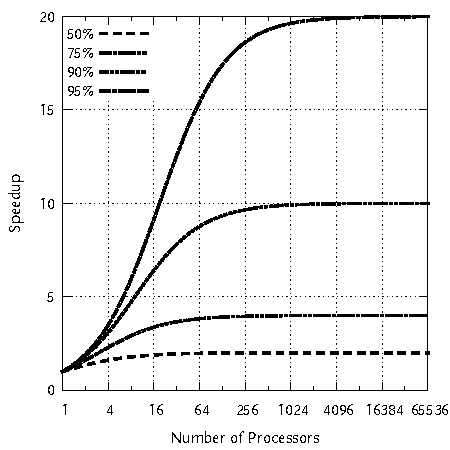
\includegraphics[scale=0.955]{pix/introduction/amdahl}}
	\hfill % alternativ auch \hspace{1cm} für genaue Angaben
		\subfloat[Gustafson's law]{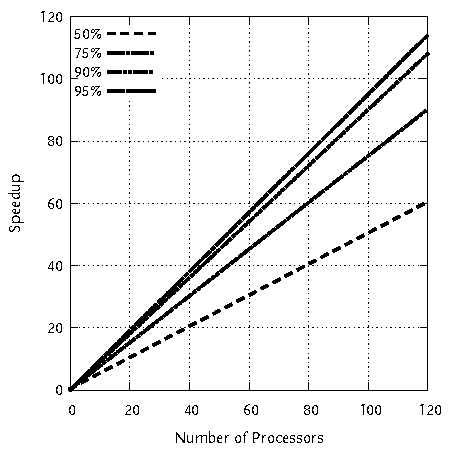
\includegraphics[scale=0.955]{pix/introduction/gustafson}}
	%\hfill %
	\caption{Amdahl's law and Gustafson's law}
	\label{fig:amdahl}
\end{figure}
%
%\newpage
%\noindent
As figure \ref{fig:amdahl} implicates, Amdahl's law predicts always a possible upper limit, whereas Gustafson's law does not. The reason is the difference opinion about the used \emph{problem size}. Problem size actually means the amount of data that has to be processed. Amdahl implicates a fixed problem size, so the calculating\,/\,communication ratio for every PU decreases when more PUs are used.

Gustafson predicts that the users will usually process more data (greater problem size) when they have more machines, mainly for getting more accurate results in the same amount of time.

Both laws are valid, as they target slightly different fields under different assumptions.

\superpar
The TOP500 project \cite{top500} aims to deliver statistics about the 500 most powerful general purpose HPC clusters in the world, and the technical development of those, because it helps manufacturers and (potential) users exchanging software and data, as well as establishing collaborations. The list is updated half-yearly (november and june) since 1993 and reflects the actual evolution in computing, as the aggregated performance of the list shows characteristics of Moore's law predicting a growth in performance by factor two every 18 months. Specific data about the computers are among others the number of cores, the power consumption, the theoretical performance ($R_{peak}$) and measured performance ($R_{max}$) in TFlops ($10^{12}$\,floating point operations per second, double precision). The measurement benchmark is LINPACK, which is basically a distributed solver for dense linear equation systems allowing architecture optimizations and variable problem sizes for achieving the best possible score per cluster.

%
\begin{table}[h!t]
	\caption{Abstract TOP500 List, November 2010}
	\label{tbl:top500}
	\centering
	\begin{tabular}{clcccc}
\hiderowcolors
		\toprule
			Rank	&Computer	&Cores		&$R_{max}$	&$R_{peak}$	&Power\\
					&			&			&[TFlops]	&[TFlops]	&[kW]\\
		\midrule
\showrowcolors
			1		&Tianhe-1A	&186\,368	&2566		&4701		&4040\\
			2		&Jaguar		&224\,162	&1759		&2331		&6951\\
			3		&Nebulae		&120\,640	&1271		&2984		&2580\\
			9		&Jugene		&294\,912	&826		&1003		&2268\\
		\bottomrule
	\end{tabular}
\end{table}
%
%\newpage

%\noindent
Table \ref{tbl:top500} shows four systems of the TOP500 list from november 2010. The first three have each more than one PFlops of measured performance, but also a power consumption of more than 2.5\,MW.
Jaguar drains nearly 7\,MW! For comparison, an average personal computer without monitor needs between 50 and 100\,W (at \approx 30\,GFlops $R_{max}$), a laptop with screen needs approximately 20\,W. 

%\noindent
An example breakdown of an actual cluster node can be seen in figure\,\ref{fig:powerconsumption}. Energy saving mechanics were not available---like in almost all clusters, because the main purpose of HPC is high performance, whereas general energy saving mechanics can lead to performance degradation. This picture should be applicable for many other cluster nodes and desktop machines---perhaps with lower CPU idle power consumption and one (or even more) additional GPGPU-cards (general purpose GPU).

%
\begin{figure}[H]
	\centering
	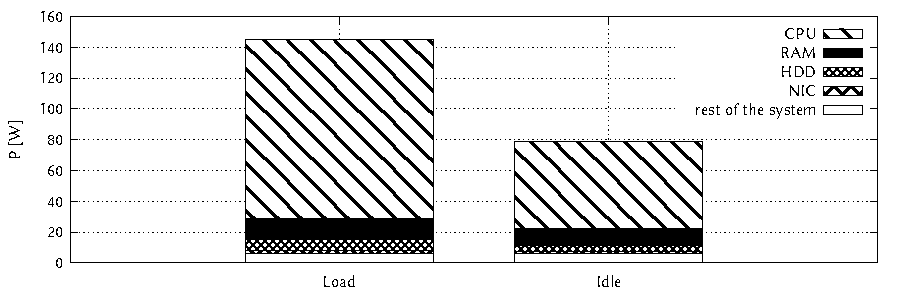
\includegraphics[width=\linewidth]{pix/systemconsumption/systemconsumption}
	\caption[System power consumption]{System power consumption\cite{minartz}}
	\label{fig:powerconsumption}
\end{figure}
%

%
%
\section{Green IT}
Like the name high performance computing implies, the goal in this area is performance. But energy efficiency gets more and more popular, as everyone seems to talk about CO$_2$ and the rising oil and energy prices. The Green500 project\cite{green500} takes the TOP500 list and reorders it considering the efficiency $\frac{MFlops}{W}$ based on $R_{max}$ and the power consumption. It is obvious by referring to table \ref{tbl:green500}, that high performance does not automatically imply energy efficiency, as the first ranked in the Green500 list delivers more than twice the energy efficiency than the first ranked in the TOP500, and more than six times than the second.
%
\begin{table}[h]
	\caption{Abstract Green500 List, November 2010}
	\label{tbl:green500}
	\centering
	\begin{tabular}{clrrr}
\hiderowcolors
		\toprule
			Rank	&Computer	&Efficiency	&Power	&TOP500 Rank\\
					&			&[MFlops/W]	&[kW]	&\\
		\midrule
\showrowcolors
			1		&NNSA/SC Blue Gene/Q Prototype	&1684.20	&39		&115\\
			11		&Tianhe-1A						&635.15		&4040		&1\\
			14		&Nebulae							&492.64		&2580		&3\\
			88		&Jaguar							&253.07		&6951		&2\\
		\bottomrule
	\end{tabular}
\end{table}
%

%\noindent
Application developers have to think about energy efficiency too, because bad program behaviour (e.\,g. polling) has impact on sleep time and the needed performance (e.\,g. algorithms) to finish a task.

But green IT means more than just energy efficiency. It is commercially relevant, as the consumer has direct advantages and a better feeling about ``helping the environment''. But even more important are the questions concerning the use of toxic materials or recyclability\,/\,reusability\,/\,refurbishability. Shamefully those topics are not well represented in mass-media, and many consumers do not even know where to dump their electronic waste. Those things are mainly handled and controlled by laws. A well-known example is ``RoHS'', which can be read on many stickers at electronic articles. RoHS stands for restriction of hazardous substances and describes limits of using toxic materials in products. Another example is the ``energy star standard'' which gives specifications about how much different devices (for example PCs or gaming consoles) are allowed to consume in active-, idle-, sleep- and standby-mode.\cite{greenIT}

%
%
\section{Goals and Structure of this Thesis}
HPC clusters need a large amount of power. Measuring this consumption for the whole cluster is very problematic, especially component measurement is only doable for few nodes, because special equipment is needed to record the consumption of a CPU or GPU. Such measurements are useful to find ways of saving energy or to predict the energy consumption after replacing components. In order to estimate at least the consumption of one of the main consumers---the CPU---a model based on its frequency and voltages will be presented and the needed data sources implemented.

\superpar
The rest of this thesis is structured as follows: 
chapter\,\ref{chap:model} deals with the calculation of the power consumption of a processor and how this can be approximated. Also some general strategies to reduce this consumption are listed.
Chapter\,\ref{chap:interfaces} lists some of the interfaces given by a modern Linux needed to get data like frequency and sleep time from a processor.
Some details about the projects that will be extended and used, as well as the actual implementation of the new features are described in chapter\,\ref{chap:implementation}.
Last but not least, chapter\,\ref{chap:evaluation} evaluates the processor model based on real world examples, and shows the functionality of the implementations.
% !TeX program = lualatex
% !TeX root = main.tex
\renewcommand*{\dictumwidth}{0.7\textwidth}
\setchapterpreamble[u]{%
	\dictum[Gordon E. Moore%\footnotemark
]{``The complexity for minimum component costs has increased at a rate of roughly a factor of two per year... Certainly over the short term this rate can be expected to continue, if not to increase. Over the longer term, the rate of increase is a bit more uncertain, although there is no reason to believe it will not remain nearly constant for at least 10 years. That means by 1975, the number of components per integrated circuit for minimum cost will be 65,000. I believe that such a large circuit can be built on a single wafer.''}}

\chapter{Modelling the Processor Power Consumption}
\label{chap:model}
\bigskip
\textit{A formula describing the power consumption of a processor using its voltage and frequency, as well as different approximations about how to calculate this consumption based on reference values will be formulated and compared in this chapter.}
%\footnotetext{\url{ftp://download.intel.com/museum/Moores_Law/Articles-Press_Releases/Gordon_Moore_1965_Article.pdf}}

\bigskip
\lettrine[lines=2, lhang=.1, lraise=.1]{A}{s} seen in the previous chapter, the cluster energy consumption depends heavily on the used CPUs. The power consumption of a CPU ($P_{total}$) consists of a dynamic ($P_{dyn}$), a leakage ($P_{leak}$) and a short circuit power consumption ($P_{short}$). Additionally, recent processors include more and more components being formerly part of the mainboard. Those components are separated from the cores and are called ``uncore''. The main reasons for this are latency reduction (integration of the memory-controller), power efficiency (separate power control unit) and better scalability with many cores. Depending on processor type, uncore includes e.\,g. the memory-controller, L3 cache or PCIE-links. Of course the power consumption depends on the number of cores, too.
%
\begin{align}
P_{total} &= \#cores \cdot ( P_{dyn} + P_{leak} + P_{short} ) + uncore\nonumber
\end{align}
%
The uncore part of the chip drains between 4\,W and 20\,W. There is by now no generic formula to calculate the power consumption of the uncore-part, and measurement can only be done with special equipment\cite{ht4uCPU}. For these reasons, uncore is considered to be constant and added to the mainboard power consumption.\\[4em]
%
Back to the main components of $P_{total}$:
%
\begin{description}
	\item[$P_{short}$] is the power caused by a short-circuit current which flows from the supply to ground during a transition period of input signals when transistors are momentarily on at the same time. Short-circuit current increases with slower signal transition times\cite{HOT96}.

``The short circuit power consumption occurs only during signal transitions and is negligible''\,\cite{martin}.

	\item[$P_{leak}$] is the gradual loss of energy from charged capacitors or when current leaks out of the intended circuit. $P_{leak}$ is modelled differently depending on the actual research and application \cite{martin, power, temp}. It is possible that leakage power drains up to 20\,\% of $P_{total}$. So, further model improvements could include $P_{leak}$, because of its temperature dependency: $ P_{leak}\,\propto \, T^2 \cdot V$ \cite{tempaware}.
	\item[$P_{dyn}$] is the power used to actually charge and discharge the capacitance, composed of gate and interconnect capacitance.
%
The greater this dynamic switching current is, the faster capacitive loads can be charged and discharged, enabling a better performing circuit.
\end{description}

\noindent
Nowadays $P_{dyn}$ dominates\cite{power} and modelling the processor power consumption can be done with 
\begin{itemize}
	\item $U$, the supply voltage (often referred as $CPU$ $V\kern-0.3em core$ or $V_{DD}$) [V],
	\item $f$, the frequency the processor runs at [Hz]
\end{itemize}
and
\begin{itemize}
	\item $\alpha$, an activity factor (not all gates are always switched),
	\item $C$, the capacitance at the gate outputs [F].
\end{itemize}
%
So actually, $P_{short}$ and $P_{leak}$ will be ignored and only $P_{dyn}$ considered, 
%
\begin{align}
O(P_{dyn}) &\in O(P_{dyn} + P_{leak} + P_{short}). \nonumber
\end{align}
%
Which leads to an accurate estimation of the power consumption a processor core is using\,\cite{minartz}:
%
\begin{align}
P_{core} &\approx P_{dyn}\nonumber\\
&= U^2 \cdot f \cdot \alpha \cdot C\label{eq:main}
\end{align}
%
$U$ is the dominating factor, which means power consumption reduces linear by decreasing the frequency, whereas decreasing the voltage reduces the power consumption quadratically.

By writing about ``processor power consumption'' in this thesis, it is always meant per core and without uncore.

%
%
\section{Voltage²-frequency}
The factors $\alpha$ and $C$ from the previously introduced power consumption formula\,\eqref{eq:main} are depending on many different influences like processor type, workload or temperature. To avoid measuring\,/\,guessing $C$ and $\alpha$, they are considered constant at equal workloads on a given processor:
%
\begin{align}
const &= \alpha \cdot C \nonumber \\
\Rightarrow P &= U^2 \cdot f \cdot const \nonumber \\
%
\intertext{%
Having measured two (or more) power consumptions $P_{1}$ and $P_{2}$ at different voltages ($U_1$, $U_2$) respectively frequencies ($f_1$, $f_2$) of a processor results in an easy transformation equation:}
%
\label{eq:V2f}
const &= \frac{P}{U^2 \cdot f} \nonumber \\
\Rightarrow P_{2} &= P_{1} \cdot \frac{U^2_2}{U^2_1} \cdot \frac{f_2}{f_1}
\end{align}
%
The estimated power consumption of a processor $P_{2}$ can be calculated by having a reference value triple $P_{1}$, $U_1$ and $f_1$, and the new voltage $U_2$ and frequency $f_2$, without having to deal with the actual activity $\alpha$ respectively capacitance $C$.

\section{Approximations}
\label{sec:approximations}
%\todo{ähnlich einleiten bei den subs}
Sometimes there is no possibility to measure the voltage. Either the mainboard has no interfaces for software, only \lstinline!root! can use them or there is no adequate software installed\,/\,available.

In the following subsections are approximations described dealing without or only partial\,/\,general information about the supply voltages.

\subsection{Frequency³ Approach}
\label{sec:freq3}
If no access to any voltages is available, a simplifying approach is to assume, that changing the voltage also requires to change the frequency at the same amount. Generally speaking $f_{max}$ $\propto$ $U$. This leads to $U = \beta \cdot f$, where $\beta$ is another constant\,\cite{efficientserverclusters}.
%
\begin{align}
	P &= U^2 \cdot f \cdot const \nonumber \\
	U &= \beta \cdot f \label{eq:ubetaf} \\
	\nonumber \\
	\Rightarrow P &= f^3 \cdot const \nonumber \\
	\Rightarrow P_{2} &= P_{1} \cdot \frac{f^3_2}{f^3_1}\label{eq:f3}
\end{align}
%
In contrast to equation\,\eqref{eq:V2f}, the power consumption consists only of the former and the recent frequencies ($f_1$ and $f_2$).

\subsection{Extending Approximation}
\label{sec:approx}
The connection between the voltage, the frequency and the actual power consumption is unfortunately a bit more complicated, especially at lower voltages. From \cite{power} it is known, that 
\begin{align*}
f_{max} \, \propto \, \frac{(U_{supply} - U_{threshold})^2}{U_{supply}},
\end{align*}
where $U_{supply}$ is the supply voltage and $U_{threshold}$ the threshold voltage.
The threshold voltage at the gate is needed to prevent the creation of current from the drain to the source of the transistor. If $U_{supply}$ is bigger than $U_{threshold}$ the transistor is on, and vice versa. 

In order to lower $U_{supply}$, there is a constraint to reduce $U_{threshold}$ too. But a reduction of $U_{threshold}$ means, that $P_{leak}$ (and therefore $P_{core}$) rises, because of $P_{leak} = I_{leak} \cdot U_{supply}$ and the proportionality $I_{leak} \propto \exp(−U_{threshold} \cdot \frac{q}{kT})$\cite{vt}.

While this knowledge does not help to improve the approximation directly, it does help focusing on the problems.
%
\begin{figure}[h]
	\centering
	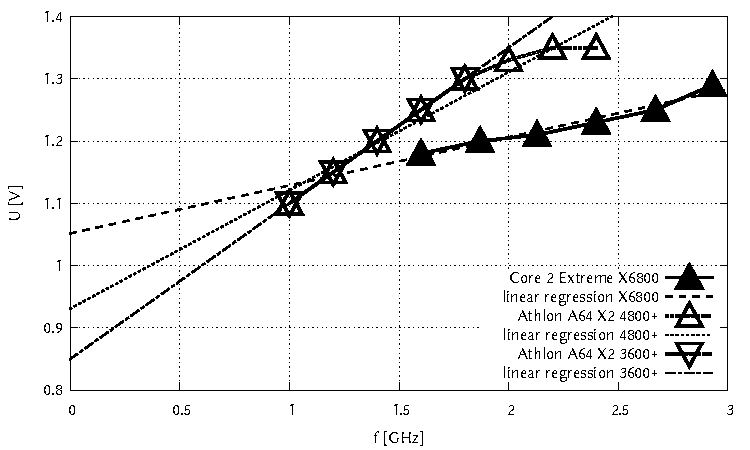
\includegraphics[width=\linewidth]{pix/pstates/pstates}
	\caption{P-state trend lines}
	\label{fig:pstates}
\end{figure}

%\noindent
In picture \ref{fig:pstates} are some valid $f$\,/\,$U$-pairs from more or less recent CPUs and a linear regression line for each.
It seems that $U$ and $f$ actually are in a linear relationship. But they are not proportional towards each other. The equation should rather be $U = \beta \cdot f + \gamma$, whereas $\beta$ is the gradient and $\gamma$ the y-intercept. Replacing $U$ results in
%
\begin{align}
	P &= U^2 \cdot f \cdot const \nonumber \\
	U &= \beta \cdot f + \gamma \label{eq:Ubetagamma}\\
	\nonumber \\
	\Rightarrow P &= (\beta \cdot f + \gamma)^2 \cdot f \cdot const \nonumber \\
	\Rightarrow P_{2} &= P_{1} \cdot \frac{f_2}{f_1} \cdot \frac{(\beta \cdot f_2 + \gamma)^2}{(\beta \cdot f_1 + \gamma)^2}
\end{align}
%
It can be seen in figure\,\ref{fig:pstates} that $\beta$ and $\gamma$ are different for every processor type. In order to calculate them, there has to be at least two valid $f$\,/\,$U$-pairs. Equation\,\eqref{eq:Ubetagamma} results directly in
%
\begin{align}
	\Rightarrow \beta &= \frac{\Delta U}{\Delta f} \qquad\text{and}\\
	\Rightarrow \gamma &= U_1 - f_1 \cdot \frac{\Delta U}{\Delta f}
\end{align}
%
By having introduced two new constants $\beta$ and $\gamma$ in equation\,\eqref{sec:freq3}, there is the option to eliminate one of them. 

Maybe it is easier to think about a y-intercept\,[$U$] than a gradient\,[$\frac{U}{f}$], but the actual choice depends, as always, on the use case.

\subsection{Intercept $\gamma$ Approach}
\label{sec:intercept}
Disappearing of $\beta$ starts again from equation\,\eqref{eq:Ubetagamma}:
%
\begin{align}
	\frac{U - \gamma}{f} &= \beta \nonumber \\
	\frac{U_1 - \gamma}{f_1} &= \frac{U_2 - \gamma}{f_2} \nonumber \\
	\Rightarrow U_2 &= U_1 \cdot \frac{f_2}{f_1} + \gamma \cdot (1 - \frac{f_2}{f_1})\label{eq:intercept}
\intertext{Inserting $U_2$ in the main equation\,\eqref{eq:V2f} results in}
	P_{2} &= P_{1} \cdot \frac{(U_1 \cdot \frac{f_2}{f_1} + \gamma \cdot (1 - \frac{f_2}{f_1}))^2}{U^2_1} \cdot \frac{f_2}{f_1} \nonumber \\
	&= P_{1} \cdot \frac{(U_1 + \gamma \cdot (\frac{f_1}{f_2} - 1))^2}{U^2_1} \cdot \frac{f_2^3}{f_1^3}
\end{align}
%
In contrast to equation\,\eqref{eq:f3} there is now an additional factor involved, which is greater 1 when $f_1 > f_2$ and lesser 1 when $f_1 < f_2$---in contrast to approach\,\ref{sec:freq3} more power drainage by switching to lower speeds, less by higher speeds. It becomes $1$ by equality of $f_1$ and $f_2$ resulting in $P_1=P_2$. 

\subsection{Gradient $\beta$ Approach}
Analogue to subsection\,\ref{sec:intercept}, $\gamma$ will vanish and the result becomes part of the main equation\,\eqref{eq:V2f}.
%
\begin{align}
	U - \beta \cdot f &= \gamma \nonumber \\
	U_1 - \beta \cdot f_1 &= U_2 - \beta \cdot f_2 \nonumber \\
	\Rightarrow U_2 &= U_1 - \beta \cdot (f_1 - f_2) \label{eq:gradient} \\
\nonumber \\
	P_{2} &= P_{1} \cdot \frac{(U_1 - \beta \cdot (f_1 - f_2))^2}{U^2_1} \cdot \frac{f_2}{f_1}
\intertext{In order to stay consistent with the equations of the other approximations, altering above equation for sake of simplicity produces:}
	P_{2} &= P_{1} \cdot \frac{(U_1 \cdot \frac{f_1}{f_2} - \beta \cdot (\frac{f_1^2}{f_2} - f_1))^2}{U^2_1} \cdot \frac{f_2^3}{f_1^3} \nonumber
\end{align}
%
but equation\,\eqref{eq:gradient} should rather be used for real-world application.

\superpar
As seen, the two extended approximations from section\,\ref{sec:approx} both need $U_1$ and the gradient $\beta$ or the intercept $\gamma$, in addition to $f_1$ and $f_2$. Nevertheless, there is no reason to use the first approximation from section\,\ref{sec:freq3}. $U_1$ can be seen in the BIOS (basic input output system) while booting, or asking the admin\,/\,support for its value. For $\beta$ or $\gamma$ some average values could be used. This should deliver acceptable results, as a short comparison shows.
\label{sec:summary}
%
\begin{figure}[!hb]
	\centering
	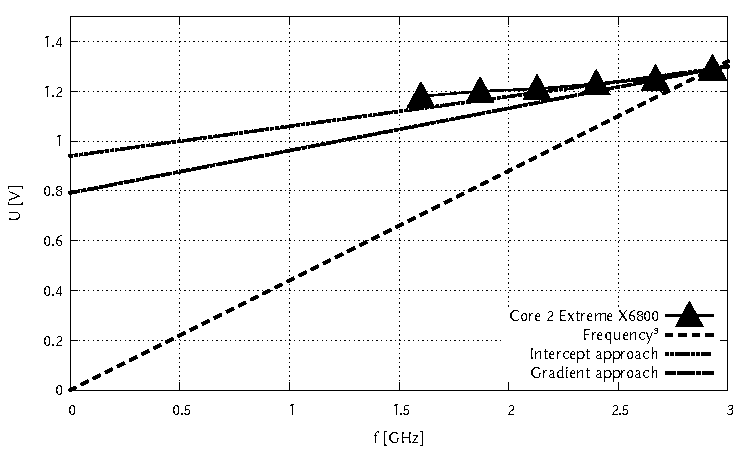
\includegraphics[width=\linewidth]{pix/modelcompare/modelcompare}
	\caption[Comparison between the approximations]{Comparison between the approximations ($\beta = 0.17$, $\gamma = 0.94$)}
	\label{fig:modelcompare}
\end{figure}
%

\noindent
Figure \ref{fig:modelcompare} shows a comparison between the three approximations discussed above at an example processor (taken from table \ref{tbl:approximations}), mean values for $\beta = 0.17$ and $\gamma = 0.94$ and the following derived formulas:

%
\begin{align*}
\text{Frequency³ approach \eqref{eq:ubetaf}} &\Rightarrow U_2 = U_1 \cdot \frac{f_2}{f_1}\\
\text{Intercept approach \eqref{eq:intercept}} &\Rightarrow U_2 = U_1 \cdot \frac{f_2}{f_1} + \gamma \cdot (1 - \frac{f_2}{f_1})\\
\text{Gradient approach \eqref{eq:gradient}} &\Rightarrow U_2 = U_1 - \beta \cdot (f_1 - f_2)\\
\end{align*}
%
It is obvious that the frequency³ approach is not able to compete against the other two. The assumption $f \, \propto \, V$ can not be considered at lower frequencies, resulting in too low estimated power consumptions.


%\newpage
%
%
\section{Power Saving Techniques}
As pointed out in this chapter, processors need much energy when calculating, and there is a great potential of reducing the power consumption of them. Power saving is implemented in hardware and in software, as those two have to work closely together in order to save the most energy without performance degradation.

%
\begin{description}
\item[Dynamic Voltage and Frequency Scaling] is the direct consequence from this chapter and possibly the most known technique. Based on its utilization the processor decreases its frequency and voltage in order to decrease power consumption too---the processor should only be as fast as needed, and therefore use as low power as possibly.\label{item:dvfs}

Mobile devices like notebooks or smart-phones use DVFS already a long time, since they notably rely on low energy consumption. Nowadays, DVFS is widespread among desktop PCs and server, and latterly some HPC cluster are using it too.

%
\begin{figure}[hbt]
	\centering
	\newcommand*\Captiontext{DVFS in multicore-processors}
	%\hfill %
		\subfloat[DualCore shared Freq \& Vcore]{% !TeX program = lualatex
% !TeX root = ../../main.tex
\begin{tikzpicture}[every node/.style={text centered}]
		\draw (0em, 0em)		node[rectangle, draw, text width=3.5em, minimum height=3.5em]
				{\large{Core 0}}
			(4.5em, 0em)	node[rectangle, draw, text width=3.5em, minimum height=3.5em]
				{\large{Core 1}}

			
			(2.25em, -2.4em)	node[rectangle, draw, text width=8em, minimum height=1.3em, fill=gray!20]
				{\small{Freq}}
			(2.25em, -3.7em)	node[rectangle, draw, text width=8em, minimum height=1.3em, fill=gray!40]
				{\small{Vcore}}
;
\end{tikzpicture}}
	\hfill % alternativ auch \hspace{1cm} für genaue Angaben
		\subfloat[QuadCore half-split Freq, shared Vcore]{% !TeX program = lualatex
% !TeX root = ../../main.tex
\begin{tikzpicture}[every node/.style={text centered}]
	\draw 	(0, -1.5em)		node[rectangle, draw, text width=3.5em, minimum height=3.5em]
				{\large{Core 0}}

			(4.5em, -1.5em)		node[rectangle, draw, text width=3.5em, minimum height=3.5em]
				{\large{Core 1}}

			(0, -5em)		node[rectangle, draw, text width=3.5em, minimum height=3.5em]
				{\large{Core 2}}
			(0, -6.65em)	node[rectangle, draw, text width=3.5em, minimum height=1.3em, fill=gray!20]
				{\small{Freq}}

			(4.5em, -5em)		node[rectangle, draw, text width=3.5em, minimum height=3.5em]
				{\large{Core 3}}
			(4.5em, -6.65em)	node[rectangle, draw, text width=3.5em, minimum height=1.3em, fill=gray!20]
				{\small{Freq}}
			(2.25em, -7.95em)	node[rectangle, draw, text width=8em, minimum height=1.3em, fill=gray!40]
				{\small{Vcore}}
;
\end{tikzpicture}}
	\hfill % alternativ auch \hspace{1cm} für genaue Angaben
		\subfloat[QuadCore split Freq \& Vcore]{% !TeX program = lualatex
% !TeX root = ../../main.tex
\begin{tikzpicture}[every node/.style={text centered}]
	\draw 	(0, 0)		node[rectangle, draw, text width=3.5em, minimum height=3.5em]
				{\large{Core 0}}
			(0, -2.4em)	node[rectangle, draw, text width=3.5em, minimum height=1.3em, fill=gray!20] 
				{\small{Freq}}
			(0, -3.7em)	node[rectangle, draw, text width=3.5em, minimum height=1.3em, fill=gray!40] 
				{\small{Vcore}}

			(4.5em, 0)		node[rectangle, draw, text width=3.5em, minimum height=3.5em]
				{\large{Core 1}}
			(4.5em, -2.4em)	node[rectangle, draw, text width=3.5em, minimum height=1.3em, fill=gray!20]
				{\small{Freq}}
			(4.5em, -3.7em)	node[rectangle, draw, text width=3.5em, minimum height=1.3em, fill=gray!40]
				{\small{Vcore}}

			(0, -6.5em)		node[rectangle, draw, text width=3.5em, minimum height=3.5em]
				{\large{Core 2}}
			(0, -8.9em)	node[rectangle, draw, text width=3.5em, minimum height=1.3em, fill=gray!20]
				{\small{Freq}}
			(0, -10.2em)	node[rectangle, draw, text width=3.5em, minimum height=1.3em, fill=gray!40]
				{\small{Vcore}}

			(4.5em, -6.5em)		node[rectangle, draw, text width=3.5em, minimum height=3.5em]
				{\large{Core 3}}
			(4.5em, -8.9em)	node[rectangle, draw, text width=3.5em, minimum height=1.3em, fill=gray!20]
				{\small{Freq}}
			(4.5em, -10.2em)	node[rectangle, draw, text width=3.5em, minimum height=1.3em, fill=gray!40]
				{\small{Vcore}}
;
\end{tikzpicture}}
	%\hfill %
	\caption[\Captiontext]{\Captiontext}
	\label{fig:dvfs}
\end{figure}
%

But DVFS has some disadvantages. 
\begin{itemize}
\item It only reduces $P_{dyn}$, but $P_{leak}$ will grow strongly in the future\cite{temp} due to further miniaturization.
\item As shown in figure \ref{fig:dvfs}, voltage and frequency can not always be free chosen. This is heavily processor and architecture dependent.
\item It takes time (and energy) to switch to another frequency-\,/\,voltage-level. Wrong decisions in switching can either harm performance respectively power saving, and there is still no ``crystal ball'' available.
\end{itemize}

\item[``Sleeping''] is used when a core has no work to do. This is done by deactivating parts of the core (ALUs, caches) or the complete core itself via clock-\,/\,power-gating, meaning to lower or even cut the frequency or the voltage. There exist different sleep states; the ``deeper'' the sleep the less power is consumed, but the longer it takes to wake up. A core can not execute instructions while sleeping.
\label{item:sleeping}

The disadvantages are mainly the same as for DVFS\cite{anand}.

\item[Idle-aware Scheduling] describes the idea of scheduling the processes in such a way, that many cores can sleep deeply.
This has to be done by the OS in order to gain the most of DVFS and sleeping.

This can of course mean some performance loss as processes have to use the same resources on a core. The opposite idea is to spread the processes on many cores for more performance and faster responses, but higher power consumption\cite{scheduler}.

\item[Intel Turbo Boost\,/\,AMD Turbo Core] Both Intel and AMD have implemented automatic overclocking features into their newer CPUs increasing their maximum frequency when the thermal budget is not yet reached. This is mainly the case, when single-threaded applications only stress individual cores. In this case, the other cores can sleep---their thermal budget is unused.
It is controversial calling dynamic overclocking a power saving technique, because the power consumption increases disproportionate to the performance gain.

Nevertheless it could help reducing the power consumption, because the faster some work is done, the longer the cores can sleep. The OS is also able to schedule processes longer on less cores when they ran faster, affecting again the sleep time of the remaining cores.

Turbo Boost\,/\,Turbo Core is all done hardware-side and transparent to the OS. By now, the only possibility for the OS\,/\,user to check if Turbo Boost\,/\,Turbo Core is in use is counting the CPU-cycles\cite{turboboost}.
\end{description}
% !TeX program = lualatex
% !TeX root = main.tex
\renewcommand*{\dictumwidth}{0.5\textwidth}
\setchapterpreamble[u]{%
	\dictum[Bill Gates%\footnotemark
]{``One thing I find myself wondering about is whether we shouldn't try and make the `ACPI' extensions somehow Windows specific. [\dots]

Or maybe we could patent something related to this.''}}
\chapter{Interfaces}
\label{chap:interfaces}
\bigskip
\textit{In this chapter, there will be a basic introduction to the different used interfaces in order to trace the processor states, beginning with ACPI, following cpufreq and cpuidle.}
%\footnotetext{\url{http://antitrust.slated.org/www.iowaconsumercase.org/011607/3000/PX03020.pdf}}

\bigskip
\lettrine[lines=2, lhang=.1, lraise=.1]{M}{odern} computer systems have plenty of ways to interact with the hardware. Of course they need to, in order to provide a fully functional and working system. The main communication between the OS and the hardware (or their firmware) is hidden for the normal computer user. But application programmer can access hardware, either direct or with one of the many generic kernel subsystems hiding hardware details and providing the main hardware functions.

%
%
\section{Advanced Configuration and Power Interface}
\label{sec:acpi}
The Advanced Configuration and Power Interface (ACPI) is a specification describing hard- and software interfaces for the implementation of OS based power management (OSPM), where the OS controls the ``power saving features'' of the devices. This is necessary considering that only the OS has all the information to efficiently send devices to sleep without harming the performance. ACPI is the successor of APM (Advanced Power Management), where only the devices themselves could control their energy saving features.

ACPI even defines its own source and machine languages: the ``ACPI Source Language'' (ASL) and the ``ACPI Machine Language'' (AML).

ACPI defines different levels of operation (operating states), composed of a letter and a number. The letter defines the region of operation and the number is an indication of the saved energy; the higher the number the more power will be saved, but latency returning to a ``lower number'' increases\cite{acpi}.\\[2em]

\noindent
Here is a short overview of the system states and what they mean:

\begin{description}
\item[G-states] Global system state definitions
	\begin{description}
	\item[G0] Working
	\item[G1\,=\,S-states] Sleeping\\
The computer appears off, but power consumption is not zero. OS context is saved and work can be resumed without rebooting.

The common sleep-states are known under suspend-to-disk (``hibernation'') and suspend-to-memory (``standby''), where the OS context is saved to disk or RAM.
	\item[G2\,=\,S5] Soft Off\,/\,Standby\\
Power consumption is minimal. No OS context is saved---system must be restarted to return to working state.
	\item[G3] Mechanical Off\\
Power consumption is zero by means of a mechanical switch. The system can be disassembled safely.
	\item[Legacy] is only used while booting or when the OS is not capable of ACPI. The device then uses its own power policy, similar to APM.
	\end{description}
\item[D-states] Device power state definitions\\device states can be applied to nearly any device on any bus. They range from D0 (Fully-On) to D3 (Off). The meaning of the states in-between is defined by each device class, and may not be defined at all. They can be thought of S-states for devices.
\item[P-states] Device and processor performance state definitions\\
	Today, P-states in processors are generally the specification of DVFS. Table \ref{tbl:pstates} shows examples for P-states.
	\begin{description}
	\item[P0] Delivers the most performance, but consumes also the most power.
	\item[Pn] Processors and devices can define up to 16 P-states, all with the same idea of limiting performance in order to save power.
	\end{description}
\item[C-states] Processor power state definitions\\
	Practically the S-states for the processor
	\begin{description}
	\item[C0] Processor is executing instructions---it is not sleeping.
	\item[Cn] different processors may implement different C-states. They can also differ in the implementation of the same state. All together is the general characteristic that a higher number implies lower power consumption but a longer wakeup-time. Not all processors report all their C-states to the OS.
	\end{description}
\end{description}
%
\newpage
\noindent
Figure \ref{fig:acpi} shows an overview of these states and how they interact which each other.

%
\begin{figure}[h]
	\centering
%	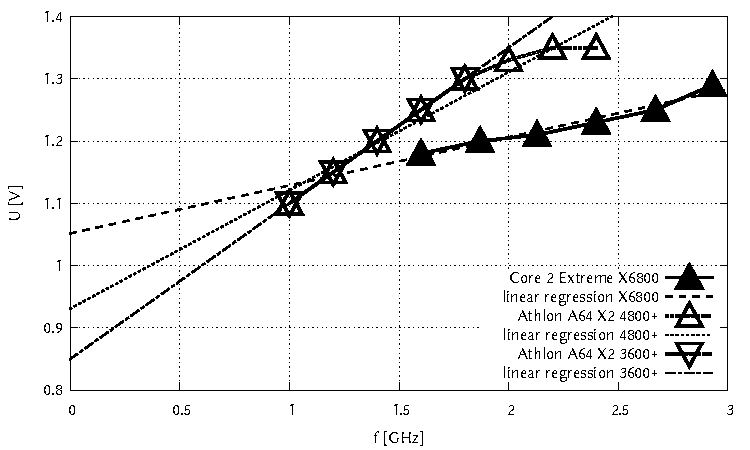
\includegraphics[width=\linewidth]{pix/pstates/pstates}
	% !TeX program = lualatex
% !TeX root = ../../main.tex
\begin{tikzpicture}[shorten >=1pt, thick, out=10, in=170, relative]
\draw 	(0,0) node[circle, minimum size=5em, inner sep=5pt, draw] (L) {Legacy}
		(5em,5em) node[circle split, minimum size=5em, inner sep=5pt, draw] (G3) 
			{G3 \nodepart{lower} \small{Mech Off}}
		(5em,-5em) node[circle split, minimum size=5em, inner sep=5pt, draw] (G2) 
			{G2 (S5) \nodepart{lower} \small{Soft Off}}
		(10em,0) node[circle split, minimum size=5em, inner sep=5pt, draw] (G0) 
			{G0 (S0) \nodepart{lower} \small{Working}}
		(13em,5em) node (Power) 
			{\small{Power Off}}
		(20em,0) node[circle split, minimum size=5em, inner sep=5pt, draw] (G1)
			{G1 \nodepart{lower} \small{Sleeping}}


		(0,-10em) node[circle split, minimum size=5em, inner sep=5pt, draw] (C0)
			{C0 (Px) \nodepart{lower} \small{CPU}}
		(10em,-10em) node[circle, minimum size=5em, inner sep=5pt] (C1)
			{\ldots}
		(20em,-10em) node[circle split, minimum size=5em, inner sep=5pt, draw] (Cn)
			{Cn \nodepart{lower} \small{CPU}}
;
\begin{scope}[circle, node distance=0em and 0em]
		\node[above right=of G1, draw] (S1) {S1};
		\node[right=of G1, draw] (S2) {S2};
		\node[below right=of G1, draw] (S3) {S3};
		\node[below=of G1, draw] (S4) {S4};

%		\node[above left=of C0, draw] (P0) {P0};
%		\node[left=of C0, draw] {\vdots};
%		\node[below left=of C0, draw] {Pn};
\end{scope}

		\draw[->] (G1) to node[below, sloped] {\small{Wake Event}} (G0);
		\draw[->] (L) to (G0);
		\draw[->] (G0) to (L);
		\draw[->] (G2) to (L);
		\draw[<-] (L) to (G3);
		\draw[->] (G3) to (G0);
		\draw[->] (G0) to (G2);
		\draw[->] (G2) to (G0);
		\draw[->] (G0) to (G1);
		\draw[<-] (G3) to (Power);

		\draw[->] (C0) to (C1);
		\draw[->, out=15, in=165, relative] (C0) to (Cn);
		\draw[->] (C1) to (Cn);
		\draw[->] (C1) to (C0);
		\draw[->, out=15, in=165, relative] (Cn) to (C0);
		\draw[->] (Cn) to (C1);
\end{tikzpicture}
\newcommand*\Captiontext{ACPI state transition overview}
	\caption[\Captiontext]{\Captiontext\cite{acpi}}
	\label{fig:acpi}
\end{figure}
%

%
\begin{table}[h]
	\caption[P-state examples]{P-state examples\cite{techarp}}
	\label{tbl:pstates}
	\centering
	\begin{tabular}{lccc}
\hiderowcolors
		\toprule
			&Core 2 Extreme X6800&Athlon A64 X2 4800+&Athlon A64 X2 3600+\\
			&[GHz / V]&[GHz / V]&[GHz / V]\\
		\midrule
\showrowcolors
			P0&2.93 / 1.2875&2.4 / 1.350&1.8 / 1.30\\
			P1&2.67 / 1.2500&2.2 / 1.350&1.6 / 1.25\\
			P2&2.40 / 1.2250&2.0 / 1.325&1.4 / 1.20\\
			P3&2.13 / 1.2125&1.8 / 1.300&1.2 / 1.15\\
			P4&1.87 / 1.2000&1.6 / 1.250&1.0 / 1.10\\
			P5&1.60 / 1.1750&1.4 / 1.200&--\\
			P6&--&1.2 / 1.150&--\\
			P7&--&1.0 / 1.100&--\\
		\bottomrule
	\end{tabular}
\end{table}
%

%
%
\section{CPUFreq}
CPUFreq is the generic kernel subsystem for managing processor P-states and was merged in kernel 2.6.9. It aims to provide a clean interface, where architecture-specific details (driver) are isolated from the generic power management policies (governor).\cite{cpufreq, ondemand}

%
\subsection{Driver}
Drivers are the interface to the processor. They must implement specific functions, like listing the available target frequencies or the frequency-change-mechanism. Providing information about the processor, e.\,g. the transition latencies or the minimum\,/\,maximum frequencies, is a duty of the driver, too. These informations are either hard-coded and general, or retrieved through the MSR of the processor. ``Machine Specific Registers'' or ``Model Specific Registers'' are a direct interface to the CPU for configuration and getting information. They can only be accessed with root-privileges and are, as the name suggests, processor dependent. MSR can be used with the assembly instructions \lstinline!RDMSR! (reads MSR) or \lstinline!WRMSR! (writes MSR).

As driver are very processor dependent, they also have to check weather they can work with the given CPU or not.

%
\subsection{Governor}
Governor are fully driver-independent and the power management policies that decide when\,/\,if to change the processor frequency.

The following governor are merged into the kernel and deliver quite a variety of policies to chose from.

\subsubsection{Performance}
The ``performance''-governor sets the CPU statically to the highest frequency within the borders of \lstinline!scaling_min_freq! and \lstinline!scaling_max_freq!.

\subsubsection{Powersave}
The ``powersave''-governor sets the CPU statically to the lowest frequency within the borders of \lstinline!scaling_min_freq! and \lstinline!scaling_max_freq!.

\superpar
The ``performance''- and ``powersave''-governors are not changing the frequency. They can be useful in some situations---hot summers or phases where latency is crucial---but they essentially disable DVFS by locking the frequency.

\subsubsection{Userspace}
The ``userspace''-governor allows the user, or any userspace program running with UID \lstinline!root!, to set the CPU to a specific frequency by making a sysfs file \lstinline!scaling_setspeed! available.

\subsubsection{Ondemand}
The ``ondemand''-governor aggressively sets the CPU depending on the current usage. It mainly switches to the highest frequency in order to complete the task and then switches instantly to the lowest. This tactic is also called ``race-to-idle''. To do this the CPU must have the capability to switch the frequency very quickly.

\subsubsection{Conservative}
The ``conservative''-governor, much like the ``ondemand''-governor, sets the CPU depending on the current usage.  It differs in behaviour in that it gracefully increases and decreases the CPU speed rather than jumping to the maximum speed the moment there is any load on the CPU. This behaviour is more suitable in a battery powered environment. 

\superpar
The ``ondemand''- and ``conservative''-governors have some preferences controlling their behaviour. These so called tuneables can be found in the CPUFreq-sysfs interface found in the appendix\,\ref{sec:cpufreqsysfs}.

%
\subsection{Programming interface}
CPUFreq also offers a C\,/\,C++ programming interface by including \lstinline!<cpufreq.h>! and linking against the \lstinline!libcpufreq!-library.

The following listing shows an abstract from the interface-specification used later in the implementation.
%
\begin{lstlisting}[%
	language=C,%
	caption={libcpufreq abstract},%
	%label={lst:freq},%
	numbers=left,%
	firstnumber=68]
/* determine current CPU frequency
 * - _kernel variant means kernel's opinion of CPU frequency
 * - _hardware variant means actual hardware CPU frequency,
 *    which is only available to root.
 */

extern unsigned long cpufreq_get_freq_kernel(unsigned int cpu);
extern unsigned long cpufreq_get_freq_hardware(unsigned int cpu);
\end{lstlisting}


% *
% * returns 0 on failure, else frequency in kHz.

%
%
\section{CPUIdle}
Like CPUFreq ``controls'' the P-states, CPUIdle is the generic kernel subsystem managing the C-states reported by ACPI---some BIOS hide deeper C-states. The maximum number of C-states the Linux kernel can handle can be found under \lstinline!/proc/acpi/processor/*/power!, for example \lstinline!max_cstate:C8!. This value represents not the number of C-states implemented in the used hardware\cite{powertop}. CPUIdle was merged in kernel 2.6.24. Exactly like CPUFreq it separates architecture-specific details (driver) from the architecture-independent implementation (governor).\cite{cpuidle, cpuidlepaper, lwn:cpuidle, cpuidle:intel}

The following governor are merged into the kernel.

\subsubsection{ladder}
The ``ladder''-governor works fine with periodic tick-based kernels. It checks every tick if it can go in a deeper idle state or not. This step-wise model works not very well with tickless kernels, because without a periodic timer tick it may not get a chance to use a deeper idle state whenever it goes idle.

\subsubsection{menu}
The ``menu''-governor on the other hand can handle this. It looks at different parameters like what the expected sleep time is (as provided by the tickless kernel), latency requirements, previous C-state residency and \lstinline!max_cstate! requirement and then picks the deepest possible idle state straight away.

%
\subsection{sysfs}
Global information can be found under\\[1em]
%
\noindent
\lstinline!$ ls -l /sys/devices/system/cpu/cpuidle!
\begin{multicols}{2}
\begin{itemize}
\renewcommand{\labelitemi}{\drsh}
\item \lstinline!current_driver!\\
	name of the current driver
\item \lstinline!current_governor_ro!\\
	name of the current governor
\end{itemize}
\end{multicols}
%

\noindent
Specific information per CPU X can be found under\\[1em]
%
\noindent
\lstinline!$ ls -l /sys/devices/system/cpu/cpuX/cpuidle!
%
\begin{multicols}{2}
\begin{itemize}
\renewcommand{\labelitemi}{\drsh}
\item \lstinline!state0!
\item \lstinline!state1!
\item \lstinline!state2!
\item \lstinline!state3!
\end{itemize}
\end{multicols}
%

\newpage
\noindent
\lstinline!$ ls -l /sys/devices/system/cpu/cpuX/cpuidle/state0!
%
%\todo{looks a bit empty, and the following description is hard to read due to the descriptive names}
%
%There are some descriptive files, like \lstinline!desc! and \lstinline!name! containing name of and description about the idle state. The exit latency is kept in \lstinline!latency!, while the consumed power, the total time spent in this state and the number of times this state was entered are in \lstinline!power!, \lstinline!time! and \lstinline!usage!.
%
\begin{multicols}{2}
\begin{itemize}
\renewcommand{\labelitemi}{\drsh}
\item \lstinline!desc!\\
	idle state description
\item \lstinline!latency!\\
	latency time exiting this state, in microseconds
\item \lstinline!name!\\
	idle state name
\item \lstinline!power!\\
	power consumed in this state
\item \lstinline!time!\\
	time spent in this state, in microseconds
\item \lstinline!usage!\\
	number of times this state was entered
\end{itemize}
\end{multicols}
%

\superpar
Figure~\ref{fig:cpufreqidle} gives a simple overview over the CPUFreq- and CPUIdle-framework, pointing out the general similarity. Up to now, these two frameworks are working absolutely independent from each other\cite{scheduler}.
%
\begin{figure}[ht]
	\centering
	%\hfill %
		\subfloat[CPUIdle]{% !TeX program = lualatex
% !TeX root = ../../main.tex
\begin{tikzpicture}[every node/.style={text centered}]
		\draw (0em, -2em)		node[draw, fill=gray!20%]
, text width=11em, minimum height=3.5em]
				{driver interface}

			(0em, 2em)		node[draw, fill=gray!20%]
, text width=11em, minimum height=3.5em]
				{governor interface}

			(0em, 0em)		node[draw, fill=white%]
, text width=10em, minimum height=2em] (cpuidle)
				{CPUIdle-infrastructure}



			(-4em, 4em)		node[draw, fill=white%]
, minimum height=2em] (ladder)
				{ladder}			
			(-4em, 5.5em)	node[font=\itshape] {step-wise}


			(4em, 4em)		node[draw, fill=white%]
, minimum height=2em] (menu)
				{menu}			
			(4em, 5.5em)	node[font=\itshape] {latency-based}




			(9em, 4em)	node {governors}
			(9em, -4em)	node {driver}
			
			(-2.5em, -4em)	node[draw%]
, minimum height=2em, fill=white] (acpiidle)
				{acpi-cpuidle}




			(0em, -7em)	node[draw%]
, minimum height=2em, fill=white] (acpidriver)
				{ACPI driver}

			(4em, -4em)	node[draw%]
, minimum height=2em, fill=white] (haltidle)
				{halt\_idle}
;

	\draw[->, line width=1.3pt] (4.5em, 3em) -- (4.5em, 1em);%(menu) -- (cpuidle);
	\draw[->, line width=1.3pt] (-4.5em, 3em) -- (-4.5em, 1em);%(ladder) -- (cpuidle);

	\draw[<-, line width=1.3pt] (4em, -3em) -- (4em, -1em);%(haltidle) -- (cpuidle);
	\draw[<-, line width=1.3pt] (-4em, -3em) -- (-4em, -1em);%(acpiidle) -- (cpuidle);
	\draw[<-, line width=1.3pt] (acpidriver) -- (acpiidle);
\end{tikzpicture}}
	\hfill % alternativ auch \hspace{1cm} für genaue Angaben
		\subfloat[CPUFreq]{% !TeX program = lualatex
% !TeX root = ../../main.tex
\begin{tikzpicture}[every node/.style={text centered}]
		\draw (0em, -2em)		node[draw, fill=gray!20%]
, text width=12em, minimum height=3.5em]
				{driver interface}

			(0em, 2em)		node[draw, fill=gray!20%]
, text width=12em, minimum height=3.5em]
				{governor interface}

			(0em, 0em)		node[draw, fill=white%]
, text width=11em, minimum height=2em] (cpuidle)
				{CPUFreq-infrastructure}



			(-5.5em, 4em)		node[draw, fill=white%]
, minimum height=2em] (ondemand)
				{ondemand}			
			(-5.5em, 5.5em)	node[font=\itshape] {aggressive}


			(5.5em, 4em)		node[draw, fill=white%]
, minimum height=2em] (conservative)
				{conservative}			
			(5.5em, 5.5em)	node[font=\itshape] {battery-fair}

			(0em, 4em)		node[draw, fill=white%]
, minimum height=2em] (userspace)
				{userspace}	



%			(-11em, 4em)	node {governors}
%			(-11em, -4em)	node {driver}
			
			(-4em, -4em)	node[draw%]
, minimum height=2em, fill=white] (acpifreq)
				{acpi-cpufreq}

(3.5em, -4em)	node[draw%]
, minimum height=2em, fill=white] (speedstep)
				{speedstep}



			(0em, -7em)	node[draw%]
, minimum height=2em, fill=white] (acpidriver)
				{ACPI driver}
			
;

	\draw[->, line width=1.3pt] (5em, 3em) -- (5em, 1em);%(menu) -- (cpuidle);
	\draw[->, line width=1.3pt] (-5em, 3em) -- (-5em, 1em);%(ladder) -- (cpuidle);

	\draw[<-, line width=1.3pt] (4em, -3em) -- (4em, -1em);%(haltidle) -- (cpuidle);
	\draw[<-, line width=1.3pt] (-4em, -3em) -- (-4em, -1em);%(acpiidle) -- (cpuidle);
	\draw[<-, line width=1.3pt] (acpidriver) -- (acpifreq);
	\draw[<-, line width=1.3pt] (acpidriver) -- (speedstep);
\end{tikzpicture}}
	%\hfill %
	\caption[Design Overview CPUIdle\,/\,CPUFreq]{Design Overview CPUIdle\,/\,CPUFreq\cite{overview}}
	\label{fig:cpufreqidle}
\end{figure}
%

%
%
\section{Intelligent Platform Management Interface}
IPMI enables system administrators to manage computer systems and monitor their operation through a set of standardized computer system interfaces.

It is possible to communicate with a distant computer over a serial connection or a local network with IPMI. Error messages can be sent with SNMP (simple network management protocol). Direct BIOS access over LAN is also possible.

The interfaces are working independently from any OS and allow system administration without installed OS or even in standby-mode. More possibilities arise while the computer system is running, for example starting\,/\,stopping the computer, or disabling the on-\,/\,off- or reset-button.

The core of IPMI is the so called baseboard management controller (BMC). Other Controller for monitoring special hardware can be connected to it over the IPMB (intelligent platform management bus). This way monitoring fan speeds or the voltages of CPUs can be done mainly by hardware with low performance impact on the OS or other running software.
The BMC is already integrated on recent server mainboards\cite{ipmi}.

%Open source management software for IPMI exists:
%IPMItool (BSD-Lizenz)
%GNU FreeIPMI (GPL)


\superpar
While IPMI focuses on remote maintenance and large data centers with special hardware, lm-sensors\footnote{\url{http://www.lm-sensors.org/}} concentrates on providing off-the-shelf hardware monitoring support for Linux. Lm-sensors is widely used in private servers and small test clusters made up of standard PC components.

The minimum update interval of lm-sensors is only 1.5 seconds, whereas IPMI is event-based and can deliver sensor data within 50\,milliseconds. For that reason, and because most recent clusters are using IPMI, integration of lm-sensors has low priority.
% !TeX program = lualatex
% !TeX root = main.tex
\renewcommand*{\dictumwidth}{0.5\textwidth}
\setchapterpreamble[u]{%
	\dictum[Verity Stob%\footnotemark
]{``The primary duty of an exception handler is to get the error out of the lap of the programmer and into the surprised face of the user.''}}
\chapter{Implementation}
\label{chap:implementation}
\bigskip
\textit{After seeing the needed interfaces in the last chapter, there will be a description about the overall software environment and which components had to be modified in order to implement the processor P- and C-state tracing.}
%\footnotetext{\url{http://www.regdeveloper.co.uk/2006/01/11/exception_handling/page2.html}}

\bigskip
\lettrine[lines=2, lhang=.1, lraise=.1]{T}{he} extended programs are parts of a whole software environment developed at the ``Research Group Parallel and Distributed Systems'' (PVS). The projects intend to create and visualize trace files. A trace file is the record of the actions a program does respectively how it interacts with its environment.

The \emph{ResourcesUtilizationTracingLibrary} captures the component utilization from the OS, for example the used RAM or the transfer rates of the NIC, whereas the \emph{PowerTracingLibrary} uses an external power meter to record the power consumption of the node. The \emph{HDMPIwrapper} keeps track of MPI calls and utilizes the \emph{Trace Writing Library} to actually write the traces to the hard drive. These projects are running while the observed MPI program runs, meaning they have some performance impact and are therefore implemented in the programming language C. The performance influence differs between 0.60\,\% (500\,ms) and 10.34\,\% (20\,ms)\cite{krempel} and is mainly based on the interval length the tracing library is waiting until it records a new trace point.

Additionally, there exist projects written in Java in order to evaluate the trace files. \emph{HDTraceFormat} is used to read and modify trace files and \emph{Sunshot} can visualize them. \emph{HDPowerEstimation} can calculate the consumed energy and is able to estimate power savings based on different reschedule strategies. This shows the potential effect of activating power saving mechanisms in a cluster. HDPowerEstimation provides computed savings and pre-after-power curves.

ResourcesUtilzationLibrary will be able to trace P- and C-states, a power estimator---in the future merged into HDPowerEstimation---will be able to read these states and use them, exampled in a new strategy.

\newpage
\noindent
Figure \ref{fig:wrapper} depicts the software environment and how the described components are interacting with each other.

%
\begin{figure}[h!]
	\centering
%	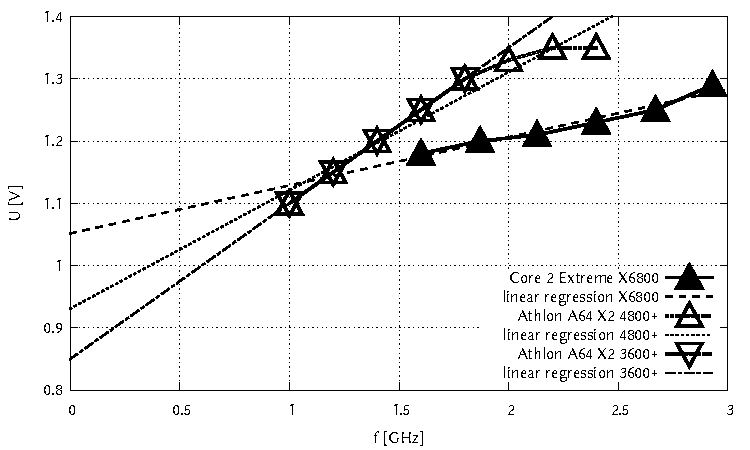
\includegraphics[width=\linewidth]{pix/pstates/pstates}
	% !TeX program = lualatex
% !TeX root = ../../main.tex
\begin{tikzpicture}
\draw 	(0,-1em) node[inner sep=5pt, minimum width=15em, minimum height=2em, draw] (PM) {Power Meter}

		(-6em,4em) node[rectangle split, rectangle split parts=2, inner sep=5pt,draw] (N1) {OS \nodepart{second} Node}
		(-2em,4em) node[rectangle split, rectangle split parts=2, inner sep=5pt,draw] (N2) {OS \nodepart{second} Node}
		(2em,4em) node[rectangle split, rectangle split parts=2, inner sep=5pt,draw] (N3) {OS \nodepart{second} Node}
		(6em,4em) node[rectangle split, rectangle split parts=2, inner sep=5pt,draw] (N4) {OS \nodepart{second} Node}

		(0,14.5em) node[inner sep=5pt, minimum width=29em, minimum height=10em, draw] (W) {Wrapper}

		(0,11.5em) node[inner sep=5pt, minimum width=15em, minimum height=2em, draw] (PMP) {Parallel MPI Program}
		(0,17.5em) node[inner sep=5pt, minimum width=15em, minimum height=2em, draw] (TWL) {Trace Writing Library}
		(-9em,14.5em) node[inner sep=5pt, minimum height=2em, text width=8em, draw] (PTL) {Power Tracing Library}
		(9em,14.5em) node[inner sep=5pt, minimum height=2em, text width=9em, draw] (RUTL) {Resources Utilization Tracing Library}

		(0,21.5em) node[inner sep=5pt, minimum width=4, minimum height=2em, draw] (TF) {Trace Files}

%		(11.5em,21.5em) node[inner sep=5pt, minimum width=4, minimum height=2em, draw] (XF) {XML File}

		(0,25em) node[inner sep=5pt, minimum width=4, minimum height=2em, draw] (HDTF) {HDTraceFormat}

		(11.5em,29em) node[inner sep=5pt, minimum width=4, minimum height=2em, draw] (HDPE) {HDPowerEstimation}
		
%		(-11.5em,29em) node[inner sep=5pt, minimum width=6em, minimum height=2em, draw] (JFC) {JFreeChart}

		(-11.5em,25em) node[inner sep=5pt, minimum width=6em, minimum height=2em, draw] (HDJ) {Sunshot}

;
		\draw[<-, line width=1.3pt] (-6em,0em) -- (N1);
		\draw[<-, line width=1.3pt] (-2em, 0em) -- (N2);
		\draw[<-, line width=1.3pt] (2em, 0em) -- (N3);
		\draw[<-, line width=1.3pt] (6em, 0em) -- (N4);

		\draw[<->, line width=1.3pt] (-6em, 9.5em) -- (N1);
		\draw[<->, line width=1.3pt] (-2em, 9.5em) -- (N2);
		\draw[<->, line width=1.3pt] (2em, 9.5em) -- (N3);
		\draw[<->, line width=1.3pt] (6em, 9.5em) -- (N4);

		\draw[line width=2.2pt, line join=miter] (-7.35em, 5.5em) -- (-7.35em, 7.5em) -- (-7em, 7.5em);
		\draw[->, line width=2.2pt] (-7.35em, 7.5em) -| (RUTL);
		\draw[line width=2.2pt] (-3.35em, 7.5em) -- (-3.35em, 5.5em);
		\draw[line width=2.2pt] (0.65em, 7.5em) -- (0.65em, 5.5em);
		\draw[line width=2.2pt] (4.65em, 7.5em) -- (4.65em, 5.5em);

		\draw[->, line width=2.2pt] (PM) -| (PTL);
		\draw[->, line width=1.3pt] (TWL) -- (TF);
		\draw[<->, line width=1.3pt] (TF) -- (HDTF);
		\draw[<-, line width=1.3pt] (HDTF) |- (HDPE) node[midway, above, pos=0.8, text width=10em, font=\fontsize{10}{11}\selectfont] {Component Estimated Energy Consumption};
		\draw[->, line width=1.3pt] (HDTF) -| (HDPE) node[midway, above left, text width=6em, font=\fontsize{10}{11}\selectfont] {Node Energy Consumption};
%		\draw[dotted, line width=1.3pt] (XF) -- (HDPE) node[midway, below right, text width=6em, font=\fontsize{10}{11}\selectfont] {Component Utilization};

%		\draw[dotted, <-, line width=1.3pt] (JFC) -- (HDPE) node[midway, above, pos=0.8, text width=10em, font=\fontsize{10}{11}\selectfont] {Component Estimated Energy Consumption};
		\draw[<-, line width=1.3pt] (HDJ) -- (HDTF);
\end{tikzpicture}
\newcommand*\Captiontext{Tracing environment at the PVS cluster}
	\caption[\Captiontext]{\Captiontext\cite{minartz}}
	\label{fig:wrapper}
\end{figure}
%

%


\section{ResourcesUtilizationTracingLibrary}
\label{sec:rutl}
The basic workflow of the library consists of an initialization phase and the tracing phase. In the initialization phase, it checks which values should be traced based on the options marked in the \lstinline!struct rutSources_s! and then writes these values into the header of the trace file.
\newpage
\begin{lstlisting}[%
	language=C,%
	caption={Frequency tracing activated?},%
	%label={lst:freq},%
	numbers=left,%
	firstnumber=152]
if(!cpufreq_available()){
	tracingData->sources.CPU_FREQ_X = 0;
	INFOMSG("Could not find cpufreq!");}
if (tracingData->sources.CPU_FREQ_X){
	for (int i = 0; i < tracingData->staticData.cpu_num; ++i){
		ret = snprintf(strbuf, RUT_STRING_BUFFER_LENGTH, "CPU_FREQ_CPU%d", i);
		ADD_VALUE(group, strbuf, INT64, "Hz", "CPU_FREQ");
}	}
\end{lstlisting}
%
\lstinline!cpufreq_available()! checks if the sysfs interface for CPUFreq is available. If not, frequency tracing will be deactivated and an info message posted. Otherwise a unique string for every CPU will be composed and added to the traced values, along with some information like the datatype \lstinline!INT64! and the unit \lstinline!"Hz"! (in contrast to \lstinline!"%"! for percentage).

The implementation for CPUIdle is analogue.

%\superpar
The tracing phase is similar, but instead of saying how the value is called and its type, the actual value is written. After every iteration, the library checks if it should stop or continue, and then waits for the length of the interval, until it begins to trace again.

The actual frequency tracing is easy, because CPUFreq offers a shared library implementing the basic functionality.
%
%\begin{lstlisting}[%
%	language=C,%
%	caption={Frequency tracing},%
%	label={lst:freq},%
%	numbers=left,%
%	firstnumber=565]
%if (tracingData->sources.CPU_FREQ_X){
%	for (int i = 0; i < tracingData->staticData.cpu_num; ++i){
%		valuei64 = (gint64) (cpufreq_get_freq_kernel(i));
%		WRITE_I64_VALUE(tracingData, valuei64);
%		DEBUGMSG("CPU_FREQ_%d = %d kHz", i, valuei64);
%}	}
%\end{lstlisting}
%
\lstinline!cpufreq_get_freq_kernel(unsigned int core)! returns the frequency of the given core. Voltage tracing is not yet implemented. This will be done based on IPMI. Because every frequency can be mapped to a corresponding voltage, frequency tracing is sufficient for evaluation. Voltages can be gathered by reading the processor manual or using software like k10ctl or c2ctl\footnote{\url{http://www.ztex.de/misc/}}.

CPUIdle does not (yet?) have a programming interface---there has to be done a little more than at frequency tracing. First step is to save the old C-state usage times and then get the new ones.

%
\begin{lstlisting}[%
	language=C,%
	caption={Idle tracing},%
	%label={lst:idle},%
	name=idle,
	numbers=left,%
	firstnumber=575]
if (tracingData->sources.CPU_IDLE_X){
	/* save old values */
		. . .
	/* get new values */
	get_c_state_times(
		tracingData->oldValues.c_states, 
		tracingData->staticData.cpu_num,
		tracingData->staticData.c_states_num);
\end{lstlisting}
%

\noindent
\lstinline!int get_c_state_times(unsigned long int *cstates, int cpu, int states)! is the function to get the C-states. It takes three arguments: the pointer to an array, where the times spend in the C-states are stored, and the number of cores and C-states. Basically, the function traverses the specific folders and files in the sysfs interface of CPUIdle and writes the values to the array\cite{powertop}.

Because the times the processors have spend in a state are total values since the last system start, the differences between formal and recent values are needed. Those differences are added together to get the times the cores have spend in idle (in microseconds).
\begin{align*}
	\text{\lstinline!idle_time!} &= \sum\limits_{n=1}^{\text{\lstinline!states!}} \text{time in } C_n
\end{align*}
The active time (C0) is simply the interval length (given in milliseconds) minus the the time spend in idle. There might be a small divergence, because of the precision of the function used to send the tracing thread to sleep while not tracing (``\lstinline!g_usleep()! may have limited precision, depending on hardware and operating system; don't rely on the exact length of the sleep\cite{glib}.''). 

The reason for not just taking the usage time of C0 as the active time is caused in the absence of regular updates for this variable, and these seldom updates are not representing active time. An explanation for this behaviour lays in the mode of operation of CPUIdle, as only the function responsible for sending cores to idle is updating the usage values.

%
%\begin{lstlisting}[%
%	language=C,%
%	%caption={Idle tracing},%
%	%label={lst:idle},%
%	name=idle,
%	numbers=left,%
%%	firstnumber=594
%]
%	/* difference */
%		. . .
%	/* calculating time spend in idle for every core */	
%	for (int i = 0; i < tracingData->staticData.cpu_num; ++i){
%		
%		/* total time in idle */
%			. . .		
%		/* time not in idle: easy, interval - time in idle, 
%		 * careful as time in idle is given in microsecs */
%		guint64 interval = (tracingData->interval) * 1000;
%		guint64 c0 = interval - total;
%		valuef = c0 / interval * 100.0;
%						
%		WRITE_FLOAT_VALUE(tracingData, valuef);
%		DEBUGMSG("CPU_IDLE_C%d_%d = %f%%", 0, i, valuef);
%				
%		for (int j = 1; j < tracingData->staticData.c_states_num; ++j){
%			valuef = c_states[i * tracingData->staticData.c_states_num + j] / interval * 100.0;
%					
%			WRITE_FLOAT_VALUE(tracingData, valuef);
%			DEBUGMSG("CPU_IDLE_C%d_%d = %f%%", j, i, valuef);
%}	}	}
%\end{lstlisting}

The written values are the percentages the core has spend in these states: 
\begin{align*}
\text{\lstinline!interval_length!} &= \text{\lstinline!tracingData->interval!} \cdot 1000\\
percentage\,Cn &=  \frac{\text{time in } Cn}{\text{\lstinline!interval_length!}} \cdot 100
\end{align*}

%
%
\section{Power Estimator}
The structure of the power estimator resembles CPUFreq\,/\,CPUIdle. One part is the representation of a CPU (driver), the other part is a estimation strategy (governor). The driver has to provide values like the available frequencies or the power usage in the different C-states. It also has to implement miscellaneous functions for getting and setting values, and the function \lstinline!double!\,\lstinline!getPower(int frequency, float[] c_usage)! which is used by the governor to get the recent power consumption. To read the trace files the power estimator uses HDTraceFormat.

In the provided implementation \lstinline!getPower()! uses the consumption model presented in this thesis, which is extended by the actual usage of the processor in the intervals.

%
\begin{align*}
P_{recent} &= \text{\lstinline!max_power!} \cdot \frac{frequency_{recent}}{\text{\lstinline!max_frequency!}} \cdot \frac{voltage_{recent}^2}{\text{\lstinline!max_voltage!}^2}
\end{align*}
%
%The usage of the actual utilization is based on the factor \lstinline!idle!, describing the consumption at 0\,\% utilization $P_{idle} = \text{\lstinline!max_power!} \cdot \text{\lstinline!idle!}$. The consumption at \lstinline!util!\,\% utilization is

%\begin{align*}
%P_{recent} &= P_{recent} \cdot (u + \text{\lstinline!idle!} - u \cdot \text{\lstinline!idle!})
%\end{align*}
%
\lstinline!c_usage! contains the usage of the different C-states in this interval in percent. The next step is to use this information and add the consumptions of the other C-states, stored in \lstinline!power_cstates! to finally get the power consumption in this step.

\begin{align*}
P_{recent} &= P_{recent} \cdot \text{\lstinline!c_usage[0]!}\\
P_{idle} &= \sum (\text{\lstinline!power_cstates[n]!} \cdot \text{\lstinline!c_usage[n]!})\\
P_{total} &= P_{recent} + P_{idle}
\end{align*}
%
The implemented governor now just multiplies each consumption with its interval length and accumulates all these consumptions. 

\begin{align*}
E_{total} = \sum\limits^{steps} (\text{\lstinline!getPower()!} \cdot \text{\lstinline!interval[step]!})
\end{align*}
%
The final energy consumption in Wh is $E_{total} / 3600$, because interval length is given in seconds.

A governor does not have to simply sum up all the values. It can try to implement a strategy analysing the actual or next steps and alter values to lower the needed power consumption. This scenario is useful on systems not applying any energy saving mechanisms to show a possible effect in reducing the overall power consumption.

\subsection*{Example}
A short example shows the sanity of the calculations given above. Table\,\ref{tbl:variables} shows experienced values for an example CPU.

%
\begin{table}[h!t]
	\caption{Variables for power estimator calculation example}
	\label{tbl:variables}
	\centering
	\begin{tabular}{cc}
\hiderowcolors
		\toprule
			Variable&Value\\
		\midrule
\showrowcolors
			\lstinline!power_cstates!&\{0, 5, 2, 1\}\\
			\lstinline!frequencies!&\{1833, 1333, 1000\}\\
			\lstinline!voltages!&\{1.1, 1.0, 0.9\}\\
			%\lstinline!idle!&0.75\\
			\lstinline!max_power!&100\\
		\bottomrule
	\end{tabular}
\end{table}
%

The consumption will be computed with the following values given for this interval

%
\begin{itemize}
\item \lstinline!frequency! = 1333
\item \lstinline!c_usage! = \{0.3, 0.1, 0.1, 0.5\}
%\item \lstinline!util! = 0.4
\end{itemize}
Calculation begins with the main formula based on the baseline values, which are just the values for P0.

%
\begin{align*}
P_{recent} &= 100 \cdot \frac{1333}{1833} \cdot \frac{1.0^2}{1.1^2}\\
&= 60.1
\end{align*}
%
%The result in $P_{recent}$ will be further used with the utilization information 
%
%
%\begin{align*}
%P_{recent} &= 60.1 \cdot (0.4 + 0.75 - 0.4 \cdot 0.75)\\
%&= 51.1
%\end{align*}
%
The result in $P_{recent}$ will be further used with the usage information for C0---the percentage the processor was active in this interval

%
\begin{align*}
P_{recent} &= 60.1 \cdot 0.3\\
&=18.0
\end{align*}
%
The power consumption for the active processor in this step is 18.0\,W. To get the consumption for the idle processor, the power consumption in the idle states have to be multiplied with their usage

%
\begin{align*}
P_{idle} &= 0.1 \cdot 5 + 0.1 \cdot 2 + 0.5 \cdot 1\\
&= 1.2
\end{align*}
%
Resulting in the complete power consumption in this interval

%
\begin{align*}
P_{total} &= P_{recent} + P_{idle} = 18.0 + 1.2\\
&= 19.2
\end{align*}
which seems reasonable, considering the processor was only 30\,\% of this interval active.
% !TeX program = lualatex
% !TeX root = main.tex
\renewcommand*{\dictumwidth}{0.5\textwidth}
\setchapterpreamble[u]{%
	\dictum[David H. Baley%\footnotemark
]{``12.  If all else fails, show pretty pictures and animated videos, and don't talk about performance.''}}

\chapter{Evaluation}
\label{chap:evaluation}
\bigskip
\textit{The final chapter deals with the evaluation of the processor model described in the second chapter,  as well as the evaluation of the extension to ResourcesUtilizationTracingLibrary from the previous chapter.}
%\footnotetext{\url{http://crd.lbl.gov/\,dhbailey/dhbpapers/twelve-ways.pdf}}

\bigskip
\lettrine[lines=2, lhang=.1, lraise=.1]{M}{easurements} of the different frequency\,/\,voltage-pairs (P-states) and their corresponding power consumption of the processor (without the other system) are hard to find, because special equipment is needed respectively the mainboard has to be modified\cite{ht4uCPU}. Even measurements with the complete system are mostly not qualified for serious comparisons. Either there are too few measurements or the test procedure is not really described.

One exception are so called ``over-clocking"-sites trying to seize the last bit of performance of a processor by using either big tower cooler, water cooling or even liquid nitrogen. This is done by rising the frequency and voltage of the processor until no stable operating is possible expressing in processor miscalculations, memory failures or complete system crashes.

\section{Processor Model Validation}
\label{sec:pmv}
To check the accuracy of the processor power consumption model, real world measurements were taken from \cite{xbit}. These measurements are from a variety of different systems with different frequency\,/\,voltage-pairs---no P-states because frequency and voltage were increased ``by hand''---for the whole system.

Because the essential power consumption equation (\ref{eq:V2f}, $P = U^2 \cdot f \cdot \alpha \cdot C$) only deals with the processor, not the complete system, the validation is based on the differences between the measured data-points and the calculated data-points to a baseline. This baseline is always the highest reached frequency, and therefore the highest power consumption of a test series.

The power consumption for the whole system consists obviously of the processor consumption and the consumption of the remaining system.
%
\begin{align*}
W &= P + S
\end{align*}
%
$W$ stands for the power consumption of the whole system, $P$ for the processor and $S$ for the system without processor. The test systems were stressed with the LINPACK frontend LinX producing load mainly on the processor (on all available cores) and some RAM. By assuming that the rest of the system is idle, or at least always utilized the same amount, it is possible to remove $S$ by writing

%
\begin{align*}
W_1 - W_2 &= (P_1 + S) - (P_2 + S)\\
			&= P_1 - P_2\\
			&=U_1^2 \cdot f_1 \cdot \alpha \cdot C - U_2^2 \cdot f_2 \cdot \alpha \cdot C\\
			&=\alpha \cdot C \cdot (U_1^2 \cdot f_1 - U_2^2 \cdot f_2)\\
\\
\Rightarrow W_1 - W_2 &= \delta \cdot (U_1^2 \cdot f_1 - U_2^2 \cdot f_2)
\end{align*}
%
All these values are available, except $\delta$. A little rearrangement of the equation above and building the mean value results in \delta:

%
\begin{align*}
\bar{\delta}  &= \frac{W_i - W_j}{U_i^2 \cdot f_i - U_j^2 \cdot f_j}
\end{align*}
%
Based upon these equation table\,\ref{tbl:ppcverification} shows the complete results of this examination. A mean variance of 4.30\,\% (6.55\,W) and maximum variance of 10.27\,\% (15.49\,W) is quite good, considering the measurements are based on whole systems and quite different processor types (dual-\,/\,quad-core, with and without uncore). The calculated results were mostly above the measured data indicating the rising temperature at those high frequencies as an additional influence. 

As already discussed in section\,\ref{sec:summary} the approximations are just as good as the amount of data they work with. Table\,\ref{tbl:approximations} based on the P-states of three real world processors shows an average difference of 0.039\,V (3.56\,\%) respectively 0.024\,V (2.10\,\%) for the gradient and intercept approaches, whereas the frequency³ approach is off by 0.28\,V (23.38\,\%). The reasons for this were discussed in section\,\ref{sec:approx} and lead to the other two approximations. Figure\,\ref{fig:modelcompare} depicts this fact.

%\todo{approximations auf summary verweisen, wiederholen, tabelle am ende}

%
%
\newpage
\section{P- and C-state Tracing Evaluation}
To examine the functionality of the implemented processor state tracing, a script generating a specific load pattern was used on a dual-core notebook enabling a visual check. The script can be found in the appendix \ref{sec:stress}. The notebook has three P-states (frequencies: 1000\,MHz, 1333\,MHz, 1833\,MHz), four C-states and runs the ondemand governor.

The load pattern consists of

%
\begin{multicols}{2}
\begin{description}
\item[00\,s] sleep for 10 seconds
\item[10\,s] CPU-load on core 1 for 20 seconds
\item[20\,s] CPU-load on core 2 for 20 seconds
\item[30\,s] stop stressing core 1
\item[40\,s] stop stressing core 2\\sleep for 10 seconds
\item[50\,s] writing 1024 MB to harddisk
\item[90\,s] terminating trace and script
\end{description}
\end{multicols}
%

\noindent
Figure \ref{fig:tracing} shows the visualization with Sunshot for the resulting trace. It shows well the changes of the P-states under load and the usage of the deep C-states in idle. While idle the trace reports nearly always the use of the C3-state, and never the C1- or even C2-state.

Writing to the harddisk shows an interesting picture. Usage of C3 is still very high, with some activity in C0 and idling in C2 (C1 is again unused), though the utilization of core 1 shows always 100\% and core 2 has phases of high utilization, too. 
P-state usage for core 1 is rather high, whereas core 2 is approximately half the time in the lowest P-state.

After finishing writing, the last 10 seconds show again some idle time with nearly 100\,\% C3- and lowest P-state-usage.

%Average utilization matches average frequency nearly perfect: 
%\begin{align*}
%0\,\% &\equiv 1000 \text{MHz}&100\,\% &\equiv 1833\,\text{MHz}\\
%\Rightarrow 66.67\,\% &\equiv 1555 \text{MHz}&46.40\,\% &\equiv 1387\,\text{MHz}
%\end{align*}

%\subsection*{Utilization vs. C0-usage}

\superpar
As seen in figure\,\ref{fig:tracing} utilization of one core matches always C0-usage, except while writing to harddisk. But utilization is actually the C0-usage, so they should be exactly the same.

The utilization $u_{CPU}$ in the time interval $[t_{i-1}, t_i]$ is calculated with

%
\begin{align*}
u_{CPU}(t_{i-1}, t_i) =& 1-\frac{x_{idle}(t_i) - x_{idle}(t_{i-1})}{x_{total}(t_i) - x_{total}(t_{i-1})}
\end{align*}
%
whereas $x_{idle}(t_i)$ is the time spent in idle and $x_{total}(t_i)$ the total elapsed time since system start\cite{krempel}. There is no difference in the formula which was used in section\,\ref{sec:rutl}:
%
\begin{align*}
percentage\,Cn &=  \frac{\text{time in } Cn}{\text{\lstinline!interval_length!}} \cdot 100
\end{align*}
%
$x_{idle}(t_i)$ and $x_{total}(t_i)$ are provided by libgtop\cite{libgtop}, which presents the values of \lstinline!\proc\stat!, which delivers statistics of the kernel and the system. Statistics for the CPU are the times spent in different situations since system start:

%
\begin{multicols}{2}
\begin{description}
\item[user] normal processes executing
\item[nice] niced processes executing
\item[system] processes in kernel mode
\item[idle] twiddling thumbs
\item[iowait] waiting for I/O to complete
\item[irq] servicing interrupts
\item[softirq] servicing softirqs
\end{description}
\end{multicols}
%

\noindent
While watching the tracing progress with \lstinline!vmstat!, which also uses \lstinline!\proc\stat!, idle counter stalls and \lstinline!iowait! increases, as expected. After checking the code segment of libgtop which is in charge of providing the values from \lstinline!\proc\stat!, the different results in tracing the utilization and the C0-usage are becoming clear. Libgtop reads from \lstinline!\proc\stat! and sums the values up to provide $x_{total}(t_i)$.

In order to get the full idle time, the above equation has to use $x_{iowait}(t_i)$ too.

%
\begin{align*}
u_{CPU}(t_{i-1}, t_i) =& 1-\frac%
{x_{idle}(t_i) + x_{iowait}(t_i) - x_{idle}(t_{i-1}) - x_{iowait}(t_{i-1})}%
{x_{total}(t_i) - x_{total}(t_{i-1})}
\end{align*}
%
Figure\,\ref{fig:bugfree} shows the visualization of the same load pattern with the adjusted version of the tracing library. Utilization now equals C0-usage.

% 
\begin{table}[hb]
	\caption[Tracing Statistics on notebook]{Tracing Statistics on notebook---average values across the whole trace}
	\label{tbl:statistics}
	\centering
	\begin{tabular}{*{7}{c}}
\hiderowcolors
		\toprule			
			&C0\,[\%]&C1\,[\%]&C2\,[\%]&C3\,[\%]&frequency\,[MHz]&utilization\,[\%]\\
		\midrule
\showrowcolors
			core 1&27.50&0.00&5.84&66.12&1392&26.11\\
			core 2&26.41&0.03&6.42&66.37&1375&25.66\\
		\bottomrule
	\end{tabular}
\end{table}
%



\noindent
Table \ref{tbl:statistics} shows that the coverage of the C-states is 99.46\,\% respectively 99.23\,\%. The missing 1 percent is the failure given the slightly varying interval times and of course some rounding mistakes. The difference between utilization and C0-usage is now very low, but still there. This will be rechecked after using the exact interval times.

%
\begin{sidewaysfigure}[h]
	\centering
	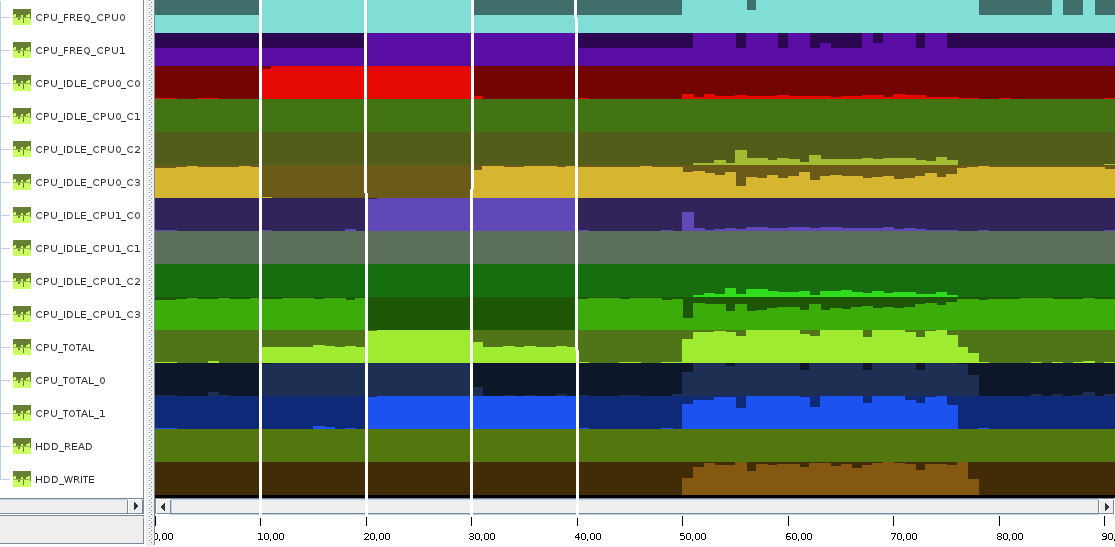
\includegraphics[width=\linewidth, height=\textheight, keepaspectratio]{pix/bug}
	\caption{Tracing screenshot showing utilization bug}
	\label{fig:tracing}
\end{sidewaysfigure}
%
\begin{sidewaysfigure}[h]
	\centering
	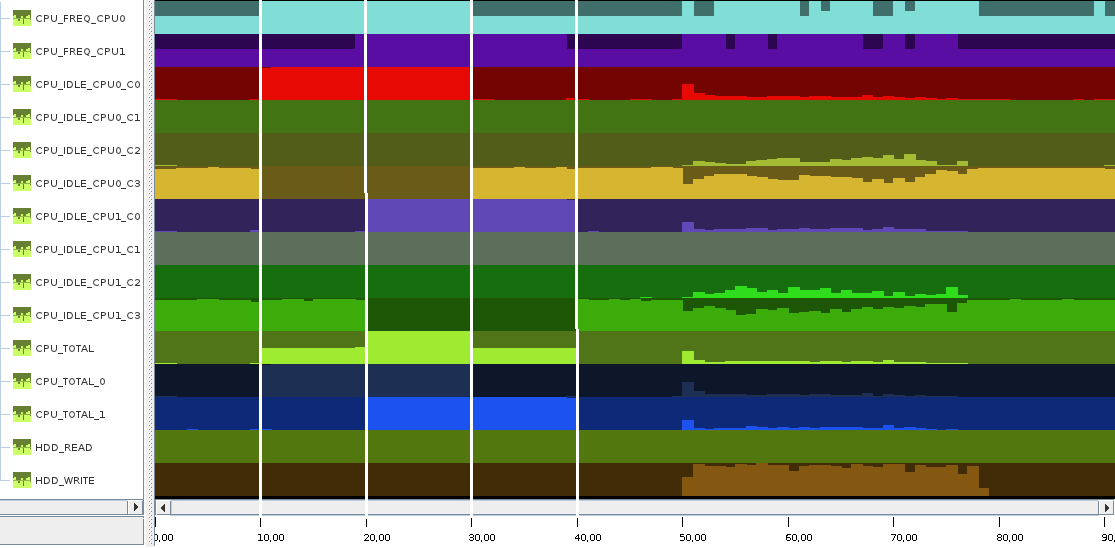
\includegraphics[width=\linewidth, height=\textheight, keepaspectratio]{pix/bugfree}
	\caption{Tracing screenshot without utilization bug}
	\label{fig:bugfree}
\end{sidewaysfigure}
%
\clearpage

%
%
%\section{Power Consumption Estimation Model}

%
%
\chapter{Conclusion and Future Work}
\enlargethispage{5\baselineskip}
Reducing power consumption is important. First step is always to measure what consumes when the most. It is usually not possible to measure every component of every node in a cluster. Because of that, a model has been presented calculating the power consumption of a processor based on its frequency and voltage. The resulting equation $P_2 = P_1 \cdot \frac{U_2^2 \cdot f_2}{U_1^2 \cdot f_1}$ needs a baseline measurement for $P_1$ at frequency $f_1$ and voltage $U_1$. The further three approximations can be used when voltage tracing is not (fully) available.
Evaluation showed this is a usable way of estimating. Taking many different overclocked systems measured with different frequency-\,/\,voltage-pairs (no P-states) resulted in a mean variance of 4.30\,\% (6.55\,W) and maximum variance of 10.27\,\% (15.49\,W) using this model. The approximations were evaluated with the P-states of three processors. The frequency³ approach, based purely on the frequency, showed a mean difference of 23.38\,\%, whereas the other two (intercept and gradient approaches) based on more information involving the characteristics of the P-states were rather good with mean differences of 3.56\,\% respectively 2.10\,\%.

In order to use this model, the appropriate values have to be recorded. To do so, an existing tracing library was extended to log the P- and C-states of a processor using the kernel subsystems CPUFreq and CPUIdle. Visual inspection and the evaluation showed reasonable results. 

A power estimator was implemented using the resulting trace files to finally gather the power respectively energy consumption of the processor based on the presented model. The estimator resembles the design of CPUFreq\,/\,CPUIdle allowing easy combination of different processor types and analysis strategies.

\superpar
Future work consists of improvements to the model by measuring the impact of the temperature change and the consumption of the uncore-part of the CPU.

ResourcesUtilizationTracingLibrary has to be further extended to include the usage of the real elapsed time for calculating the active processor time, and voltage tracing with IPMI has to be implemented.

Later improvements also include merging the power estimator into HDPowerEstimation and considering the amount of state-changes for a more detailed power consumption, as well as developing strategies to predict energy saving potential on hardware not using energy saving mechanisms.\\[1em]
All together, it shows that this approach is a reasonable and working way to estimate the power consumption used by the processor.

% Appendix (Anhänge), could have multiple chaper-files:
\appendix

% big letters
\pagenumbering{Roman}
\clearscrheadfoot 
\cfoot{\pagemark}

% !TeX program = lualatex
% !TeX root = main.tex
\chapter{Appendix}

%
%
\section*{Tables}
Table\,\ref{tbl:approximations} compares the accuracy of the three processor power consumption approximations (see \ref{sec:approx}) for three processors based on their actual P-states, based on table\,\ref{tbl:pstates}. All values are simple differences. Last column shows the total variation, based on
\begin{align*}
percentage &= \frac{\sum \text{differences}}{\sum \text{target voltages}}
\end{align*}

% 
\begin{table}[hb]
	\caption{Frequency³ vs. Gradient vs. Intercept approach}
	\label{tbl:approximations}
	\centering
	\begin{tabular}{*{9}{r}}
\hiderowcolors
		\toprule			
			&P1\,[V]&P2\,[V]&P3\,[V]&P4\,[V]&P5\,[V]&P6\,[V]&P7\,[V]&$\Delta$\,[\%]\\
		\midrule
			\multicolumn{9}{c}{Core 2 Extreme X6800}\\
		\midrule
\showrowcolors
			Frequency³\,$\Delta$&%
				-0.077&-0.170&-0.277&-0.378&-0.472&--&--&22.66\\
			Gradient\,$\Delta$&%
				-0.007&-0.028&-0.061&-0.093&-0.114&--&--&4.97\\
			Intercept\,$\Delta$&%
				0.007&0.000&-0.020&-0.038&-0.045&--&--&1.82\\
		\midrule
\hiderowcolors
			\multicolumn{9}{c}{Athlon A64 X2 4800+}\\
		\midrule
\showrowcolors
			Frequency³\,$\Delta$&%
				-0.113&-0.200&-0.288&-0.350&-0.413&-0.475&-0.538&27.38\\
			Gradient\,$\Delta$&%
				-0.034&-0.043&-0.052&-0.036&-0.020&-0.004&0.012&2.32\\
			Intercept\,$\Delta$&%
				-0.034&-0.043&-0.052&-0.037&-0.021&-0.005&0.011&2.34\\
		\midrule
\hiderowcolors
			\multicolumn{9}{c}{Athlon A64 X2 3600+}\\
		\midrule
\showrowcolors
			Frequency³\,$\Delta$&%
				-0.094&-0.189&-0.283&-0.378&--&--&--&20.09\\
			Gradient\,$\Delta$&%
				0.016&0.032&0.048&0.064&--&--&--&3.40\\
			Intercept\,$\Delta$&%
				0.010&0.020&0.030&0.040&--&--&--&2.13\\
		\bottomrule
	\end{tabular}
\end{table}
%

\superpar
\noindent
Table\,\ref{tbl:ppcverification} compares the measured power consumption with the calculated consumption based on the equations from section\,\ref{sec:pmv}.
%\newpage
% 
\begin{longtable}{*{6}{r}}
%\centering
\caption{Processor Power Consumption Verification}\label{tbl:ppcverification}\\
\hiderowcolors
\toprule			
f\,[GHz]&U\,[V]&P$_{measured}$\,[W]&P$_{calculated}$\,[W]&$\Delta$\,[W]&$\Delta$\,[\%]\\
\midrule
\endfirsthead

%
\caption*{Processor Power Consumption Verification}\\
\hiderowcolors
\toprule			
f\,[GHz]&U\,[V]&P$_{measured}$\,[W]&P$_{calculated}$\,[W]&$\Delta$\,[W]&$\Delta$\,[\%]\\
\midrule
\endhead

%
\bottomrule
\endfoot

%
%
%		\midrule

			\multicolumn{6}{c}{Athlon II X2 255}\\
		\midrule
\showrowcolors
			3.1&1.40&111.6&115.2&3.59&3.12\\
			3.2&1.40&113.1&117.2&4.13&3.52\\
			3.4&1.40&116.4&121.3&4.90&4.04\\
			3.6&1.40&120.5&125.4&4.88&3.89\\
			3.8&1.50&140.9&140.9&0.00&0.00\\
%
%
		\midrule
\hiderowcolors
			\multicolumn{6}{c}{Athlon II X4 635}\\
		\midrule
\showrowcolors
			2.9&1.40&146.3&148.8&2.44&1.64\\
			3.0&1.40&149.7&152.3&2.58&1.69\\
			3.2&1.40&156.4&159.4&2.96&1.86\\
			3.4&1.40&162.7&166.4&3.73&2.24\\
			3.5&1.50&188.3&188.3&0.00&0.00\\
%
%
		\midrule
\hiderowcolors
			\multicolumn{6}{c}{Athlon II X2 555}\\
		\midrule
\showrowcolors
			3.2&1.40&122.7&133.9&11.20&8.36\\
			3.4&1.40&125.9&137.9&11.96&8.67\\
			3.6&1.40&128.3&141.8&13.52&9.53\\
			3.8&1.40&130.8&145.8&14.97&10.27\\
			4.0&1.55&167.6&167.6&0.00&0.00\\
%
%
		\midrule
\hiderowcolors
			\multicolumn{6}{c}{Athlon II X4 965}\\
		\midrule
\showrowcolors
			3.4&1.40&186.3&195.0&8.65&4.44\\
			3.6&1.40&192.0&203.4&11.35&5.58\\
			3.8&1.40&197.5&211.8&14.26&6.73\\
			3.9&1.50&240.2&240.2&0.00&0.00\\
%
%
		\midrule
\hiderowcolors
			\multicolumn{6}{c}{Core2Duo E7600}\\
		\midrule
\showrowcolors
			3.06&1.28&95.5&101.3&5.81&5.73\\
			3.2&1.28&97.3&103.9&6.59&6.34\\
			3.4&1.28&100.6&107.6&6.98&6.49\\
			3.6&1.28&103.9&111.3&7.37&6.63\\
			3.8&1.35&116.7&123.5&6.75&5.47\\
			4.0&1.50&147.0&147.0&0.00&0.00\\
%
%
		\midrule
\hiderowcolors
			\multicolumn{6}{c}{Core2Quad Q9505}\\
		\midrule
\showrowcolors
			2.83&1.28&125.9&127.8&1.93&1.51\\
			3.0&1.28&132.6&133.4&0.78&0.59\\
			3.2&1.28&138.8&139.9&1.12&0.80\\
			3.4&1.28&145.6&146.5&0.85&0.58\\
			3.6&1.28&150.3&153.0&2.69&1.76\\
			3.8&1.35&172.3&174.6&2.26&1.29\\
			3.9&1.40&189.0&189.0&0.00&0.00\\
%
%
		\midrule
\hiderowcolors
			\multicolumn{6}{c}{Core i3-540}\\
		\midrule
\showrowcolors
			3.07&1.13&85.9&86.8&0.88&1.02\\
			3.2&1.13&88.1&88.8&0.69&0.78\\
			3.4&1.20&106.7&99.1&7.58&7.65\\
			3.6&1.20&109.6&102.6&6.96&6.78\\
			3.8&1.30&118.3&117.8&0.54&0.46\\
			4.0&1.30&120.2&121.9&1.68&1.38\\
			4.2&1.38&136.3&136.3&0.00&0.00\\
%
%
		\midrule
\hiderowcolors
			\multicolumn{6}{c}{Core i7-860}\\
		\midrule
\showrowcolors
			2.8&1.13&154.1&160.6&6.45&4.02\\
			3.0&1.13&158.5&167.9&9.40&5.60\\
			3.2&1.13&165.0&175.3&10.25&5.85\\
			3.4&1.13&170.6&182.6&11.99&6.57\\
			3.6&1.20&201.4&208.2&6.76&3.25\\
			3.8&1.20&241.7&244.1&2.40&0.98\\
			4.0&1.38&277.2&277.2&0.00&0.00\\
%
%
		\midrule
\hiderowcolors
			\multicolumn{6}{c}{Core i7-950}\\
		\midrule
\showrowcolors
			3.07&1.20&189.8&181.6&8.24&4.54\\
			3.2&1.20&203.7&188.2&15.49&8.23\\
			3.4&1.20&212.3&198.5&13.85&6.98\\
			3.6&1.20&219.9&208.7&11.22&5.38\\
			3.8&1.20&234.4&218.9&15.48&7.07\\
			4.0&1.30&264.9&264.7&0.21&0.08\\
			4.2&1.40&317.0&317.0&0.00&0.00
\end{longtable}
%

%
%
\newpage
\section*{CPUFreq sysfs}
\label{sec:cpufreqsysfs}
Governor specific information and settings can be found under\\[1em]
%
\noindent
\lstinline!$ ls -l /sys/devices/system/cpu/cpufreq/GOVERNOR!

\begin{description}
\item[ondemand] There are a number of sysfs file accessible parameters:
%
\begin{multicols}{2}
\begin{itemize}
\renewcommand{\labelitemi}{\drsh}
\item \lstinline!sampling_rate!\\
	this is how often the kernel should look at the CPU usage to make decisions on what to do about the frequency, in microseconds.

\item \lstinline!show_sampling_rate_min!\\
	The sampling rate is limited by the HW transition latency or by kernel restrictions.

\item \lstinline!up_threshold!\\
	defines what the average CPU usage between the samplings of \lstinline!sampling_rate! needs to be for the kernel to make a decision whether it should increase the frequency.  For example when it is set to its default value of 95 it means that between the checking intervals the CPU needs to be on average more than 95\,\% in use to decide that the CPU frequency needs to be increased.  

\item \lstinline!ignore_nice_load!\\
	this parameter takes a value of 0 or 1. When set to 0 (default), all processes are counted towards the
``cpu utilisation'' value.  When set to 1, the processes that are run with a ``nice'' value will not count (and thus be ignored) in the overall usage calculation.  This is useful if CPU intensive calculations are running on a laptop and it is not important how long it takes to complete.
\end{itemize}
\end{multicols}
%
\item[conservative] The governor is tweaked in the same manner as the ``ondemand''-governor through sysfs with the addition of:
%
\begin{multicols}{2}
\begin{itemize}
\renewcommand{\labelitemi}{\drsh}
\item \lstinline!freq_step!\\
	this describes what percentage steps the CPU frequency should be increased and decreased smoothly by.  By default, the CPU frequency will increase in 5\,\% chunks of the maximum CPU frequency.  It is possible to change this value to anywhere between 0 and 100, where 0 will effectively lock the CPU at a speed regardless of its load whilst 100 will make it behave identically to the ``ondemand''-governor.

\item \lstinline!down_threshold!\\
	same as the \lstinline!up_threshold! found for the ``ondemand''-governor, but for the opposite direction.
\end{itemize}
\end{multicols}
%
\end{description}
%

\newpage
\noindent
Specific information per CPU X can be found under\\[1em]
%
\noindent
\lstinline!$ ls -l /sys/devices/system/cpu/cpuX/cpufreq!
%
\begin{multicols}{2}
\begin{itemize}
\renewcommand{\labelitemi}{\drsh}
\item \lstinline!bios_limit!\\
	frequency limit as told by the BIOS.
\item \lstinline!cpuinfo_min_freq!\\
	the minimum operating frequency the processor can run at, in kHz.
\item \lstinline!cpuinfo_max_freq!\\
	the maximum operating frequency the processor can run at, in kHz. 
\item \lstinline!cpuinfo_transition_latency!\\
	the time it takes to switch between two frequencies, in nanoseconds.
\item \lstinline!cpuinfo_cur_freq!\\
	current frequency as obtained from the hardware in kHz. This is the frequency the CPU really runs at.
\item \lstinline!scaling_available_governors!\\
	available CPUFreq governors in this kernel. 
\item \lstinline!scaling_available_frequencies!\\
	available frequencies in kHz.
\item \lstinline!scaling_governor!\\
	currently activated used CPUFreq governor---``echoing'' the name of another governor changes it.
\item \lstinline!scaling_cur_freq!\\
	current frequency as determined by the governor and CPUFreq core in KHz. This is the frequency the kernel thinks the CPU runs at.
\item \lstinline!scaling_driver!\\
	used CPUFreq driver.
\item \lstinline!scaling_setspeed!\\
	if ``userspace''-governor is selected, current speed can be read here. Changing speed can be done by ``echoing'' a new frequency, but only within the limits of \lstinline!scaling_min_freq! and \lstinline!scaling_max_freq!.
\item \lstinline!scaling_min_freq!\\
	the current minimum frequency limit in kHz---``echoing'' a new value changes the limit.
\item \lstinline!scaling_max_freq!\\
	the current maximum frequency limit in kHz---``echoing'' a new value changes the limit. 
\item \lstinline!affected_cpus!\\
	CPUs that require software coordination of frequency.
\item \lstinline!related_cpus!\\
	CPUs that need some sort of frequency coordination, whether software or hardware.
\end{itemize}
\end{multicols}

%
%
\section*{Tracing Test Script}
\label{sec:stress}
The following script is used to start\,/\,stop tracing, stressing the CPU using \lstinline!stress!\footnote{\url{http://weather.ou.edu/\,apw/projects/stress/}} and writing to HDD with \lstinline!dd!. It is based on the script used in \cite{krempel}.
\lstinputlisting[language=bash, numbers=left, caption={Tracing Test Script}]{../work/RUT_2.sh}

%
%
\newpage
\section*{Tools and Software}
A bunch of great free and open tools has been used to produce this thesis:
%
\begin{itemize}
	\item \emph{\TeX works}\,\footnote{\url{http://code.google.com/p/texworks/}} for writing and \emph{lua\LaTeX}\,\footnote{\url{http://www.luatex.org/}} for producing text,
	\item \emph{LibreOffice Calc}\,\footnote{\url{http://www.libreoffice.org/}} for data analysis,
	\item \emph{Gnuplot}\,\footnote{\url{http://www.gnuplot.info/}} for plotting data and \emph{PGF/TikZ}\,\footnote{\url{http://sourceforge.net/projects/pgf/}} for generating graphics, as well as \emph{GIMP}\,\footnote{\url{http://www.gimp.org/}} for screenshot modifications,
	\item \emph{Eclipse}\,\footnote{\url{http://www.eclipse.org/}} for writing and exploring code,
	\item revision control systems \emph{git}\,\footnote{\url{http://git-scm.com/}} for code and \emph{subversion}\,\footnote{\url{http://subversion.apache.org/}} for the thesis.
\end{itemize}
 %
Fonts used in this thesis are \emph{Linux Libertine}\,\footnote{\url{http://www.linuxlibertine.org/}} as serif font, \emph{Linux Biolinum}\,\footnotemark as sans-serif font, \emph{DejaVu Sans Mono}\,\footnote{\url{http://dejavu-fonts.org/}} as monospace font and the standard math font from \emph{Computer Modern}.

%
%
\newpage
\section*{Citations}
These nice citations were used at the headings of each chapter:
\begin{description}
\item[Andreas Bogk] ``UNIX is user-friendly, it just chooses its friends.''\footnote{\url{http://chaosradio.ccc.de/cr40.html}}
%
\item[Gordon E. Moore] ``The complexity for minimum component costs has increased at a rate of roughly a factor of two per year... Certainly over the short term this rate can be expected to continue, if not to increase. Over the longer term, the rate of increase is a bit more uncertain, although there is no reason to believe it will not remain nearly constant for at least 10 years. That means by 1975, the number of components per integrated circuit for minimum cost will be 65,000. I believe that such a large circuit can be built on a single wafer.''\footnote{\url{ftp://download.intel.com/museum/Moores_Law/Articles-Press_Releases/Gordon_Moore_1965_Article.pdf}}
%
\item[Bill Gates] ``One thing I find myself wondering about is whether we shouldn't try and make the `ACPI' extensions somehow Windows specific. [\dots] Or maybe we could patent something related to this.''\footnote{\url{http://antitrust.slated.org/www.iowaconsumercase.org/011607/3000/PX03020.pdf}}
%
\item[Verity Stob] ``The primary duty of an exception handler is to get the error out of the lap of the programmer and into the surprised face of the user.''\footnote{\url{http://www.regdeveloper.co.uk/2006/01/11/exception_handling/page2.html}}
%
\item[David H. Baley] ``12.  If all else fails, show pretty pictures and animated videos, and don't talk about performance.''\footnote{\url{http://crd.lbl.gov/\,dhbailey/dhbpapers/twelve-ways.pdf}}
\end{description}
% List of figures (Abbildungsverzeichnis):
\listoffigures
% List of tables (Tabellenverzeichnis):
\listoftables
% List of listings (Codeverzeichnis):
\lstlistoflistings
% Glossary (Glossar):
%\include{Glossary}
% List of formulae (Liste der Formelzeichen):
%\include{Formulae}
% Abbreviations (Abkrzungsverzeichnis):
%\include{Abbreviations}

% References (Literaturverzeichnis):
% a) Style (with numbers: use unsrt, alpha sorted: use alpha):
\bibliographystyle{alpha}%{unsrt}
% b) The File:
\bibliography{bibliography}

\end{document}
